\documentclass[10pt,letterpaper]{article}
% Layout of an AIAA conference manuscript, built from standard packages so the draft
% compiles on a stock TeX Live (pdflatex). It follows the AIAA Technical Conference
% paper guidelines: US letter, 1 in margins, 10 pt Times, 24 pt bold title, bold
% indented abstract, centred roman-numbered section headings, lettered subsections,
% "Fig. n" / "Table n" bold captions and bracketed numeric citations.
% For the final submission, paste the body into the official AIAA template
% (new-aiaa.cls, distributed by AIAA through Overleaf); no body text depends on this file.
\usepackage[letterpaper,margin=1in]{geometry}
\usepackage[T1]{fontenc}
\usepackage[utf8]{inputenc}
\usepackage{amsmath,amssymb}
\usepackage{newtxtext,newtxmath}
\usepackage{bm}
\usepackage{graphicx}
\usepackage{xcolor}
\usepackage{booktabs}
\usepackage{array}
\usepackage{longtable}
\usepackage{siunitx}
\usepackage{algorithm}
\usepackage{algpseudocode}
\usepackage{tikz}
\usetikzlibrary{positioning,arrows.meta,fit,backgrounds}
\usepackage[numbers,sort&compress]{natbib}
\usepackage{titlesec}
\usepackage[font={small,bf},labelfont=bf,labelsep=quad]{caption}
\usepackage{enumitem}
\usepackage[hidelinks]{hyperref}

\sisetup{per-mode=symbol, detect-weight=true, group-minimum-digits=5}
\setlength{\parindent}{0.2in}
\setlength{\parskip}{0pt}
\setlist{nosep,leftmargin=0.35in}
\captionsetup[figure]{name=Fig.}
\captionsetup[table]{name=Table,position=top}
\setlength{\bibsep}{2pt}
\renewcommand{\bibfont}{\small}

% Headings: I. Section (centred), A. Subsection (bold), 1. Subsubsection (italic).
\renewcommand{\thesection}{\Roman{section}}
\renewcommand{\thesubsection}{\Alph{subsection}}
\renewcommand{\thesubsubsection}{\arabic{subsubsection}}
\makeatletter
\renewcommand{\p@subsection}{\thesection.}
\renewcommand{\p@subsubsection}{\thesection.\thesubsection.}
\makeatother
\titleformat{\section}{\normalfont\large\bfseries\centering}{\thesection.}{0.5em}{}
\titleformat{\subsection}{\normalfont\normalsize\bfseries}{\thesubsection.}{0.5em}{}
\titleformat{\subsubsection}{\normalfont\normalsize\itshape}{\thesubsubsection.}{0.5em}{}
\titlespacing*{\section}{0pt}{12pt plus 3pt minus 2pt}{6pt}
\titlespacing*{\subsection}{0pt}{9pt plus 2pt minus 2pt}{3pt}
\titlespacing*{\subsubsection}{0pt}{6pt plus 2pt minus 1pt}{2pt}

% Title block and abstract.
\newcommand{\aiaatitle}[1]{\begin{center}\fontsize{24}{28}\selectfont\bfseries #1\par\end{center}\vspace{6pt}}
\newcommand{\aiaaauthor}[1]{\begin{center}\fontsize{16}{19}\selectfont #1\par\end{center}\vspace{-6pt}}
\newcommand{\aiaaaffiliation}[1]{\begin{center}\fontsize{12}{14}\selectfont\itshape #1\par\end{center}\vspace{4pt}}
\newenvironment{aiaaabstract}
  {\begin{list}{}{\setlength{\leftmargin}{0.5in}\setlength{\rightmargin}{0.5in}\setlength{\listparindent}{0.2in}%
   \setlength{\itemindent}{0.2in}\setlength{\parsep}{0pt}}\item\relax\bfseries}
  {\end{list}\vspace{4pt}}
\newenvironment{nomenclature}
  {\section*{Nomenclature}\small\setlength{\LTleft}{0pt}\setlength{\LTpre}{0pt}\setlength{\LTpost}{0pt}%
   \begin{longtable}{@{}l@{\quad=\quad}p{0.78\textwidth}@{}}}
  {\end{longtable}\addtocounter{table}{-1}\normalsize}

% References kept whole.
\newcommand{\refalg}[1]{Algorithm~\ref{#1}}
\newcommand{\refeq}[1]{Eq.~(\ref{#1})}
\newcommand{\refeqs}[2]{Eqs.~(\ref{#1})--(\ref{#2})}
\newcommand{\reffig}[1]{Fig.~\ref{#1}}
\newcommand{\refsec}[1]{Section~\ref{#1}}
\newcommand{\reftab}[1]{Table~\ref{#1}}

% Notation.
\newcommand{\vect}[1]{\bm{#1}}
\newcommand{\mat}[1]{\mathbf{#1}}
\newcommand{\ez}{\hat{\vect{e}}_z}
\newcommand{\wb}{\vect{\omega}}
\newcommand{\mdot}{\dot{m}}
\newcommand{\Ir}{I_r}
\newcommand{\wrot}{\omega_r}
\newcommand{\wmax}{\omega_{\max}}
\newcommand{\uj}{u_j}
\graphicspath{{figures/}{../physics_simulation/figures/}}


\hypersetup{pdftitle={Convex Powered-Descent Guidance with Plant-Derived Constraints for a Jet-Vane Thrust-Vectored Electric Ducted Fan Testbed}, pdfauthor={Tang Zijian (Jacob Tang)}}
\begin{document}

\aiaatitle{Convex Powered-Descent Guidance with Plant-Derived Constraints for a Jet-Vane Thrust-Vectored Electric Ducted Fan Testbed}

{\renewcommand{\thefootnote}{\fnsymbol{footnote}}%
\aiaaauthor{Tang Zijian (Jacob Tang)\footnote{Graduate Student in Data Science, Department of Computer and Information Sciences.}}
\aiaaaffiliation{Minnesota State University, Mankato, Minnesota, 56001}}
\setcounter{footnote}{0}

\begin{aiaaabstract}
A single electric ducted fan steered by four jet vanes is a constant-mass analogue of a retro-propulsive stage, with attitude response limited by rotor angular momentum and thrust limited by battery voltage.
We present a constant-mass plant model and a guidance law that searches over fixed-duration conic programs using model-derived thrust and rate limits.
The plant bounds vane authority by jet momentum---giving a torque slope weakly dependent on lift slope at the assumed loading---couples a current-limited motor to a battery circuit, pairs intake drag with duct jet damping, and embeds an implicit-midpoint and Cayley gyrostat step in a rigid-body engine; in a torque-free, constant-speed rotor test with zero axial spin, explicit Euler amplifies transverse body kinetic energy 57-fold in \SI{2}{\second}, whereas the coupled scheme preserves it.
Of 400 dispersed starts, 355 yielded hard-terminal plans (\SI{62}{\milli\second} median); 72 had relative node gaps above \num{1e-3}, which a selective half-space repair reduced to at most \num{6.3e-4} at a 2\% median planned-energy increase.
All 400 closed-loop replica runs crossed touchdown height within \SI{0.206}{\metre\per\second} downward speed and \SI{0.333}{\metre} pad error; eight earlier rigid-body missions reached at most \SI{0.178}{\metre\per\second} immediately before contact and \SI{0.146}{\metre}. All results are simulated.
\end{aiaaabstract}

\begin{nomenclature}
$A_\parallel, A_\perp$ & axial and crossflow reference areas of the airframe, \si{\metre\squared} \\
$a$ & braking acceleration of the sink-rate envelope, \si{\metre\per\second\squared} \\
$\vect{a}$ & touchdown point (glide-slope cone apex), \si{\metre} \\
$b$ & servo error deadband, \si{\radian} \\
$C_{N_\alpha}, C_{D_0}$ & vane normal-force slope, \si{\per\radian}, and profile-drag coefficient \\
$c_k$ & epigraph variable of the energy objective at node $k$ \\
$\mat{D}$ & frame-conversion matrix $\mathrm{diag}(1,-1,-1)$ between body FRD and engine axes \\
$d$ & commanded motor duty \\
$\hat{\vect{d}}_k$ & unit thrust direction of a gapped node for the half-space floor \\
$f, f_h$ & rotor speed fraction $\wrot/\wmax$, and its value in level hover \\
$\vect{g}, g$ & gravitational acceleration vector and its magnitude, \si{\metre\per\second\squared} \\
$\vect{H}$ & rotor angular momentum $\Ir\wrot\ez$, \si{\newton\metre\second} \\
$\mat{I}, \Ir$ & body inertia tensor and rotor axial inertia, \si{\kilogram\metre\squared} \\
$K, K_\psi$ & roll/pitch and yaw vane authority at full rotor speed, \si{\newton\metre\per\radian} \\
$\ell_z, r_v$ & axial and radial vane center-of-pressure arms from the center of mass, \si{\metre} \\
$m, \mdot$ & vehicle mass, \si{\kilogram}, and jet mass flow, \si{\kilogram\per\second} \\
$N$ & number of discretization intervals on a plan leg \\
$P, P_{\max}, P_{\text{aux}}$ & electrical, maximum shaft and auxiliary power, \si{\watt} \\
$Q_a, Q_m, Q_s, \bar Q$ & aerodynamic, motor, residual-swirl and current-limit torques, \si{\newton\metre} \\
$\vect{q}, \mat{R}$ & body attitude quaternion and rotation matrix from body to world \\
$R_0, R_p$ & battery pack series and polarization resistances, \si{\ohm} \\
$\vect{r}, \vect{r}_g$ & world position ($z$ up) and landing-gate position, \si{\metre} \\
$S$ & planform area of one jet vane, \si{\metre\squared} \\
$T, T_{\max}, T_{\text{full}}, T_{\text{av}}$ & raw thrust, static ceiling, net full-speed thrust and bus-limited net thrust, \si{\newton} \\
$t_f$ & plan duration, \si{\second} \\
$\vect{u}$ & thrust acceleration $\vect{T}/m$, \si{\metre\per\second\squared} \\
$\uj$ & axial jet speed at the nozzle, \si{\metre\per\second} \\
$V, V_{\text{ref}}$ & loaded battery bus voltage and nominal reference voltage, \si{\volt} \\
$\vect{v}, v_g$ & world velocity and vertical descent speed at the gate, \si{\metre\per\second} \\
$W$ & vehicle weight $mg$, \si{\newton} \\
$\alpha_i, \alpha_{\max}, \bar\alpha$ & deflection of vane $i$, servo travel limit and controller effort limit, \si{\radian} \\
$\gamma$ & glide-slope cone half-angle from the vertical, \si{\radian} \\
$\delta_D$ & chordwise momentum fraction removed by a vane \\
$\epsilon$ & relative lossless-convexification gap \\
$\theta_{\max}$ & thrust-pointing limit from the vertical, \si{\radian} \\
$\lambda$ & vane loading parameter \\
$\rho;\ \rho_1, \rho_2$ & air density, \si{\kilogram\per\metre\cubed}; planned thrust floor and ceiling, \si{\newton} \\
$\sigma$ & slack bounding the thrust-acceleration magnitude, \si{\metre\per\second\squared} \\
$\tau_m, \tau_s, \tau_j$ & motor spool, servo and joint-drive time constants, \si{\second} \\
$\tau_t$ & normal momentum fraction removed by a vane \\
$\wb$ & body angular velocity, \si{\radian\per\second} \\
$\wrot, \wmax$ & rotor speed and its no-load maximum, \si{\radian\per\second} \\
$\omega_n, \omega_t$ & nutation frequency and planned attitude-slew bound, \si{\radian\per\second} \\
\end{nomenclature}

\section{Introduction}
\label{sec:intro}

Retro-propulsive landing asks a guidance law to place a vehicle on a pad with near-zero velocity while thrust, pointing and actuator limits all bind at once.
For classical powered descent under the losslessness hypotheses, convexification yields a second-order cone program (SOCP)~\cite{acikmese2007,acikmese2013lcvx,blackmore2016}, and the approach has flown on rocket-powered test vehicles~\cite{scharf2017}.
Whether such a controller transfers to a new vehicle depends on two things that the method itself does not supply: a plant model that is right about what limits the vehicle, and a set of planning constraints that represent those limits.
This paper addresses both for a sub-scale testbed, a \SI{3.1}{\kilogram} vehicle lifted by one \SI{90}{\milli\metre} electric ducted fan (EDF) and steered by four servo-driven jet vanes in the fan exhaust.
Small electric thrust-vectored vehicles of this kind are attractive guidance testbeds because they are cheap to fly and repeat~\cite{linsen2022}.

The vehicle is mechanically simple but differs from a rocket stage, and from the multirotors that most aerial-robot simulators target~\cite{furrer2016rotors,song2020flightmare,shah2018airsim,panerati2021gym}, in four ways.
First, the four vanes generate commanded attitude moments by redirecting the exhaust. Rotor acceleration also exerts a yaw reaction.
The vanes cannot extract more transverse momentum than the jet carries, so a thin-airfoil force law applied to each vane independently overstates their authority.
Second, the rotor stores about \SI{0.78}{\newton\metre\second} of angular momentum at hover.
Changing rotor speed exchanges angular momentum with the body, and tilting the rotor axis requires a transverse torque.
Third, the vehicle loses no mass, and its thrust ceiling is set by a motor current limit and a battery whose voltage sags under load.
Fourth, the mission simulator can apply sensor dynamics to the navigation channels. The actuator feedback channels are ideal.

These properties change the powered-descent problem.
Constant mass removes the logarithmic mass transformation. Each fixed-duration relaxation uses second-order cones for the trajectory constraints and power cones for the energy objective.
In exchange, the rotor's momentum makes thrust rate and attitude rate the binding actuator limits, and neither appears in the classical formulation.
A thrust-rate bound couples successive controls, which is outside the hypotheses under which the relaxation is known to be lossless~\cite{acikmese2011lcvx,harris2014lcvx}.
The energy that matters is electrical rather than propellant mass, and for a vehicle that hovers at 84\% of rotor speed it is dominated by the time spent airborne.

An earlier version of the project's simulator treated the vehicle loosely.
It applied independent per-vane lift forces, scaled the rotor reactions down, integrated the gyroscopic torque explicitly, and stabilized the result with a tuned angular damper.
A sequence of audits replaced each of these with a physically bounded model and a regression test.
The corrected plant has an eighth of the earlier vane authority and less than one hundredth of its damping, and the attitude law that flew the earlier plant is unstable on it.
The present guidance was developed on the corrected plant.

The contributions of this paper are as follows.
\begin{enumerate}
\item A momentum-consistent plant model for a jet-vane EDF vehicle: a control-volume vane model with a closed-form authority, a current-limited motor coupled to a battery circuit, full-strength rotor reactions, intake momentum drag with the duct's Coriolis reaction, and a coupled implicit-midpoint and Cayley integration of the body--rotor gyrostat inside a rigid-body engine that integrates gyroscopic terms explicitly (\refsec{sec:plant}).
\item A first-order-hold transcription that combines an electrical-energy surrogate with thrust, rate and sink constraints and explicit control-authority reserves (\refsec{sec:guidance}).
\item A test of the thrust-annulus relaxation over 400 dispersed starts, including a selective node-floor repair and an interval-by-interval check of physical thrust magnitude and direction rate (\refsec{sec:results-planner}).
\item A duration sweep quantifying how rapidly planned energy grows with flight time over the sampled feasible durations (\refsec{sec:results-planner}).
\item A full-state gyroscopic attitude regulator and its stability comparison with the proportional-derivative law it replaced (\refsec{sec:control}, \refsec{sec:results-attitude}).
\item A dispersed closed-loop assessment on a reduced-order replica, with paired perturbations of vane authority, rotor inertia, center of mass and planning delay (\refsec{sec:results-closedloop}).
\end{enumerate}

The scope of the evidence should be stated plainly.
Every figure in this paper is generated by a script that imports the simulator's own model and planner classes and loads the configuration files that missions load; none of those computations involves the rigid-body engine.
Closed-loop results are of two kinds.
Those that involve the rigid-body engine are taken from the project's recorded runs and are identified as recorded.
The dispersed closed-loop campaign runs the production flight computer on a reduced-order replica of the plant that omits contact and the sensor chain.
No hardware has flown.
Several model parameters are planning estimates, and \refsec{sec:limits} lists them with the bench measurements that would replace them.

\section{Related Work}
\label{sec:related}

\textit{Convex powered-descent guidance.}
A\c{c}{\i}kme\c{s}e and Ploen showed that the minimum-fuel soft-landing problem with a non-convex thrust magnitude bound has a convex relaxation whose optimum satisfies the original bound~\cite{acikmese2007}.
The result was extended to minimum landing error~\cite{blackmore2010mle}, to thrust-pointing constraints~\cite{acikmese2013lcvx}, to a general class of control constraints~\cite{acikmese2011lcvx} and, under additional conditions, to state constraints~\cite{harris2014lcvx}.
Customized interior-point solvers made the method fast enough for flight processors~\cite{dueri2017}, and it was demonstrated on a rocket-powered test vehicle~\cite{scharf2017}.
Six-degree-of-freedom problems with aerodynamic forces are non-convex and are treated by successive convexification~\cite{szmuk2018}; Malyuta et al.\ survey the field~\cite{malyuta2022convex}.
Each trial duration requires a convex solve and may require a second solve to impose thrust floors at selected nodes.
It adapts the free-final-time three-degree-of-freedom formulation to a constant-mass vehicle and examines numerically what the vehicle's rate constraints do to the tightness of the relaxation.
We solve with Clarabel, a primal-dual interior-point conic solver that supports the power cone used by the energy objective~\cite{goulart2024clarabel}.

\textit{Jet vanes and ducted fans.}
Jet-vane thrust vector control is classical in rocketry~\cite{sutton2017}, where the vane force is usually modeled with lift and drag coefficients fitted to tests or plume simulations~\cite{sung2004jetvane,liu2013jetvane}.
Ducted-fan vehicle models add momentum drag at the intake and duct-lip effects~\cite{johnson2006ducted,pflimlin2010ducted}.
Our vane model follows the momentum and angular-momentum bookkeeping of Drela's propeller formulation~\cite{drela2006qprop} and bounds each vane by its share of the jet.
Jet damping, the moment produced by the Coriolis acceleration of internal flow, is a classical rocket-dynamics result~\cite{thomson1986}.
Linsen et al.\ describe an electric small-scale rocket prototype with gimballed propulsion and optimal control~\cite{linsen2022}; the present vehicle differs in using fixed propulsion with vanes, which makes authority depend on thrust.

\textit{Simulation and structure-preserving integration.}
Common aerial-vehicle simulators model multirotors as rigid bodies with per-rotor thrust and drag torque~\cite{furrer2016rotors,song2020flightmare,shah2018airsim,panerati2021gym}, and GPU-parallel frameworks made massively parallel rigid-body simulation routine~\cite{makoviychuk2021isaac,mittal2023orbit}.
None models finite-momentum jet vanes, a stored rotor momentum that exceeds the actuator authority, or battery-limited spool dynamics.
Explicit integration of rigid-body rotation conserves neither energy nor momentum, and implicit-midpoint and Lie-group integrators that do are well established~\cite{simo1991,hairer2006,lee2007lie}.
The engine used here treats the gyroscopic term explicitly~\cite{physx2023}.
Our contribution on this point is narrow: a midpoint solve for the combined body and virtual-rotor gyrostat embedded in an engine whose integrator cannot be replaced.

\textit{Attitude control, batteries and sensors.}
The inner attitude loop uses a geometric attitude error~\cite{lee2010geometric} and a linear-quadratic regulator weighted by Bryson's rule~\cite{bryson1975}, with a backlash inverse for the servo deadband~\cite{tao1996}.
The battery is an equivalent-circuit model with one polarization branch~\cite{chen2006battery,plett2015}.
Inertial sensor errors follow Allan-variance practice~\cite{elsheimy2008allan}, the onboard attitude filter is a complementary filter~\cite{mahony2008}, and the navigation filter is an error-state Kalman filter~\cite{sola2017} with the structure of ArduPilot's EKF3~\cite{ardupilot2026ekf3}.

\section{Testbed and Simulation Architecture}
\label{sec:system}

\subsection{Vehicle}

The aerodynamic model uses a \SI{0.35}{\metre} length and \SI{0.12}{\metre} diameter for the airframe around the EDF. The asset mesh including the legs spans approximately $0.313 \times 0.313 \times 0.422$~\si{\metre}.
Four flat-plate vanes sit in the exhaust at \SI{90}{\degree} intervals.
Each vane hinges about its own radial span and is driven through \SI{\pm15}{\degree} by a hobby servo.
A differential deflection of an opposed pair produces roll or pitch, and a common-mode deflection of all four produces yaw, because the four tangential forces add around the thrust axis.
The vanes also push the vehicle sideways directly.
The controller commands five actuators: four vane angles and one motor duty.

Two propulsion profiles are modeled.
The \emph{planned 8S} profile is a 12-blade \SI{90}{\milli\metre} EDF with a KV1500 motor on an eight-cell lithium-polymer pack and a \SI{120}{\ampere} speed controller.
The \emph{legacy 6S} profile is the originally specified KV1850 unit on six cells.
All results use the 8S profile unless stated otherwise.
The 8S parts had not been purchased at the time of writing, so its parameters are planning estimates.
\reftab{tab:params} lists the parameters with the provenance each carries in the configuration files.

\begin{table}[t]
\caption{Mission-plant parameters, planned 8S profile}
\label{tab:params}
\centering
\small
\begin{tabular}{lll}
\toprule
Parameter & Value & Source \\
\midrule
\multicolumn{3}{l}{\emph{Airframe}} \\
Mass (body and four vanes) & \SI{3.104}{\kilogram} & Asset mass properties \\
Inertia $I_{xx}, I_{yy}, I_{zz}$ & 0.05, 0.05, \SI{0.02}{\kilogram\metre\squared} & Asset mass properties \\
Center-of-mass offset (FRD) & $(0,0,-0.01)$ \si{\metre} & Estimate \\
Axial, crossflow area $A_\parallel$, $A_\perp$ & 0.011, \SI{0.042}{\metre\squared} & Derived from geometry \\
Drag coefficients $C_d$, $C_{d,\perp}$ & 1.0, 1.0 & Estimate \\
Intake lip, modeled nozzle exit (FRD $z$) & \SI{-0.017}{\metre}, \SI{+0.050}{\metre} & Mesh exit at \SI{+0.055}{\metre} \\
\addlinespace
\multicolumn{3}{l}{\emph{Jet vanes}} \\
Effective vane area, travel, effort limit & \SI{0.002}{\metre\squared}, \SI{\pm0.262}{\radian}, \SI{\pm0.245}{\radian} & Rounded area, drive limits \\
Center of pressure $(r_v, 0, z_v)$ & $(0.04, 0, 0.10)$ \si{\metre} & Estimate \\
$C_{N_\alpha}$, $C_{D_0}$, $k_{\text{duct}}$ & \SI{3.5}{\per\radian}, 0.05, 1.3 & Estimate \\
\addlinespace
\multicolumn{3}{l}{\emph{Propulsion}} \\
Static thrust $T_{\max}$, net $T_{\text{full}}$ & \SI{48}{\newton}, \SI{43.07}{\newton} & Planning estimate; after neutral vane drag \\
No-load speed $\wmax$ & \SI{4649.6}{\radian\per\second} & KV $\times\ V_{\text{ref}}$ \\
Jet speed $u_{j,\max}$ & \SI{128}{\metre\per\second} & $\sqrt{2T/\rho A}$ (see \refsec{sec:limits}) \\
Shaft power $P_{\max}$ & \SI{3072}{\watt} & $T_{\max}u_{j,\max}/2$ \\
Rotor inertia $\Ir$ & \SI{2e-4}{\kilogram\metre\squared} & Estimate \\
Spool lag $\tau_m$, torque limit $\bar Q$ & \SI{0.15}{\second}, \SI{0.76}{\newton\metre} & Estimate, $K_t I_{\max}$ \\
Residual swirl fraction $f_s$ & 0.1 & Estimate \\
\addlinespace
\multicolumn{3}{l}{\emph{Servo and joint drive}} \\
Lag $\tau_s$, deadband $b$ & \SI{0.05}{\second}, \SI{0.017}{\radian} & Estimate \\
Slew, stall torque & \SI{6.98}{\radian\per\second}, \SI{1.08}{\newton\metre} & Datasheet \\
Drive stiffness, damping & \SI{80}{\newton\metre\per\radian}, \SI{2}{\newton\metre\second\per\radian} & Simulation estimate \\
\addlinespace
\multicolumn{3}{l}{\emph{Battery (8S)}} \\
Capacity, current limit, $V_{\text{ref}}$ & \SI{5}{\ampere\hour}, \SI{120}{\ampere}, \SI{29.6}{\volt} & Planned; $8\times\SI{3.7}{\volt}$ \\
Pack $R_0 = 8R_{\text{cell}}$; $R_p$, $\tau_p$ & \SI{24}{\milli\ohm}; \SI{6}{\milli\ohm}, \SI{15}{\second} & Estimate (\SI{3}{\milli\ohm}/cell; pack $R_p$) \\
Motor efficiency $\eta_m$, auxiliary power $P_{\text{aux}}$ & 0.88, \SI{10}{\watt} & Estimate \\
\bottomrule
\end{tabular}
\end{table}

\subsection{Software Architecture and Schedule}
\label{sec:architecture}

The environment is built on NVIDIA Isaac Sim~5.1 and Isaac Lab~2.3.2, which wrap the PhysX~5 engine~\cite{mittal2023orbit,physx2023}.
The vehicle is an articulation with a root body link and four vane links on revolute joints; the landing legs are collision shapes on the body.
The engine integrates only the articulated rigid bodies, the joint drives and contact.
Every other effect---actuators, propulsion, battery, aerodynamics and the rotor's angular momentum---is computed by batched tensor models in body forward-right-down (FRD) coordinates and handed to the engine as external wrenches at every physics substep.
The same code serves one mission vehicle and thousands of parallel instances.
Vectors cross between the world frame ($z$ up) and the body FRD frame in one module only, $\vect{v}^{W} = \mat{R}(\vect{q})\,\mat{D}\,\vect{v}^{F}$ with $\mat{D} = \mathrm{diag}(1,-1,-1)$.

Missions run the engine at $\Delta t = 1/120$~\si{\second} with a decimation of four, so the flight computer acts at \SI{30}{\hertz}.
\refalg{alg:substep} gives the order of operations within a substep and \reffig{fig:dataflow} the data flow.
Vane forces use the measured joint angles and link poses, not the commanded targets.
Each mission records its resolved configuration and a hash of the vehicle asset and of every simulator source and configuration file, which is how a recorded flight is tied to the plant it flew.

\begin{algorithm}[t]
\caption{One physics substep of the mission plant}
\label{alg:substep}
\small
\begin{algorithmic}[1]
\Require held action $(\alpha^{\text{cmd}}_{1..4}, d)$, engine state
\State servo update, \refeq{eq:servo}; write joint-drive targets
\State motor and battery update, \refeqs{eq:esc}{eq:energycap} $\to \wrot^{k+1}$
\State read joint angles, vane link poses, center-of-pressure velocities, body rate $\wb$
\State thrust $T=k_T\wrot^2$; spool and swirl reactions, \refeq{eq:reactions}
\State coupled jet: per-vane forces at the moving centers of pressure, \refeqs{eq:inflow}{eq:vaneforce}
\State intake drag and duct Coriolis reaction, \refeq{eq:intake}, \refeq{eq:coriolis}; body drag, \refeq{eq:bodydrag}
\State coupled midpoint predictor, \refeq{eq:midpoint} $\to$ gyroscopic torque and integration correction, \refeq{eq:correction}
\State compose all moments about the true center of mass; engine step with external forces applied once
\State \textbf{if} no contact \textbf{then} replace the engine's orientation update with the Cayley update, \refeq{eq:cayley}
\State sensor chain and navigation filter step; contact state machine update
\end{algorithmic}
\end{algorithm}

\begin{figure}[t]
\centering
\resizebox{\textwidth}{!}{%
\begin{tikzpicture}[
  node distance=4mm and 8mm,
  box/.style={draw, rounded corners=2pt, align=center, font=\scriptsize, minimum height=8mm, text width=22.8mm, fill=white},
  phys/.style={box, fill=blue!8},
  ext/.style={box, fill=orange!12},
  arr/.style={-{Stealth[length=1.6mm]}, thick},
]
\node[ext] (fc) {Flight computer\\ \SI{30}{\hertz}\\ convex plan + LQR};
\node[box, right=9mm of fc] (servo) {Servo model\\ lag, slew, deadband};
\node[box, below=of servo] (motor) {Motor + battery\\ torque, energy caps};
\node[phys, right=of servo] (drive) {Engine joint drive\\ $k=80$, $c=2$};
\node[box, right=of drive] (jet) {Coupled jet\\ 4 streamtubes, swirl};
\node[box, below=of jet] (edf) {Thrust, spool and swirl reactions};
\node[box, below=of edf] (aero) {Intake, Coriolis,\\ body drag + wind};
\node[box, right=of jet] (pred) {Coupled midpoint\\ predictor};
\node[box, below=of pred] (disp) {Wrench dispatch\\ moments about c.m.};
\node[phys, below=of disp] (physx) {Rigid-body step\\ $\Delta t = 1/120$ s};
\node[box, right=of physx] (cay) {Cayley orientation\\ (free flight)};
\node[box, above=of cay] (imu) {Sensor chain,\\ navigation filter};
\node[box, above=of imu] (contact) {Contact state\\ machine};
\draw[arr] (fc) -- node[above, font=\tiny]{$\alpha^{\text{cmd}}$} (servo);
\draw[arr] (fc.south) |- node[pos=0.75, below, font=\tiny]{duty $d$} (motor.west);
\draw[arr] (servo) -- (drive);
\draw[arr] (drive) -- node[above, font=\tiny]{$\alpha$, poses} (jet);
\draw[arr] (motor.east) -- node[below, font=\tiny]{$\wrot$} (edf.west);
\draw[arr] (motor.east) -- (jet.south west);
\draw[arr] (jet) -- (pred);
\draw[arr] (edf.east) -- (pred.south west);
\draw[arr] (aero.east) -- (disp.west);
\draw[arr] (pred) -- (disp);
\draw[arr] (disp) -- (physx);
\draw[arr] (physx) -- (cay);
\draw[arr] (cay) -- (imu);
\draw[arr] (imu) -- (contact);
\draw[arr] (contact.north) |- ++(0,4mm) -| node[pos=0.25, above, font=\tiny]{sensor estimate, contact state} (fc.north);
\begin{scope}[on background layer]
\node[draw, dashed, rounded corners, inner sep=2.5mm, fit=(servo)(motor)(drive)(jet)(edf)(aero)(pred)(disp)(physx)(cay)(imu)(contact),
      label={[font=\scriptsize]below:repeated four times per control step}] {};
\end{scope}
\end{tikzpicture}}
\caption{Data flow of one control step. The shaded orange box is the \SI{30}{\hertz} flight computer; shaded blue boxes are the rigid-body engine; white boxes are batched force and sensor models that act on it through external wrenches and joint-drive targets. Navigation channels follow the configured sensor path. Actuator feedback is ideal.}
\label{fig:dataflow}
\end{figure}

\section{Plant Model}
\label{sec:plant}

\subsection{Motor, Battery and Thrust}
\label{sec:motor}

The speed controller is modeled as a first-order speed command that a current-limited motor may or may not be able to deliver.
With $d$ the commanded duty and $V$ the loaded bus voltage, the requested acceleration and the delivered motor torque are
\begin{align}
\dot\omega_{\text{req}} &= \frac{\mathrm{clip}(d\,V/V_{\text{ref}}, 0, 1)\,\wmax - \wrot}{\tau_m}, \label{eq:esc}\\
Q_m &= \mathrm{clip}\!\left(\Ir\dot\omega_{\text{req}} + Q_a,\; -\bar Q,\; \bar Q\right), \qquad
Q_a = \frac{P_{\max}}{\wmax}\left(\frac{\wrot}{\wmax}\right)^{2}, \label{eq:motor}
\end{align}
and the rotor obeys $\Ir\dot\omega_r = Q_m - Q_a$.
The aerodynamic torque follows the momentum-theory scaling of shaft power with $\wrot^3$ and uses the same reference power as the battery load and the jet model, so the three subsystems agree on shaft power.
The model uses $\bar Q=K_t I_{\max}=\SI{0.76}{\newton\metre}$ as a motor torque cap and separately caps pack current at \SI{120}{\ampere}. Motor phase current and bus current generally differ. The no-load KV speed at \SI{29.6}{\volt} is also the reference speed for \SI{48}{\newton} gross thrust and \SI{3072}{\watt} shaft power. These effective parameters require a simultaneous loaded RPM, thrust, voltage and current measurement.
At $d = 0$ the limit is zero, as for a speed controller with the brake disabled, and the rotor coasts down on $Q_a$ with a time constant $\Ir\wrot/Q_a \approx \SI{1.7}{\second}$ at hover.
Thrust is $T = k_T\wrot^2$ with $k_T = T_{\max}/\wmax^2$.

The torque limit matters physically (\reffig{fig:spool}).
Without it, the \SI{0.15}{\second} lag stops the rotor at disarm in about \SI{0.5}{\second}, and the reaction puts \SI{5.2}{\newton\metre} on a body whose vanes hold about \SI{0.3}{\newton\metre} in yaw.
The bounded motor takes \SI{1.38}{\second} to reach hover speed from rest, compared with \SI{0.28}{\second} for the first-order lag. The cap applies to motor torque. Aerodynamic torque also slows the rotor during a speed reduction, and the isolated torque-limited trace reaches a spool reaction of \SI{0.98}{\newton\metre}.

\begin{figure}[t]
\centering
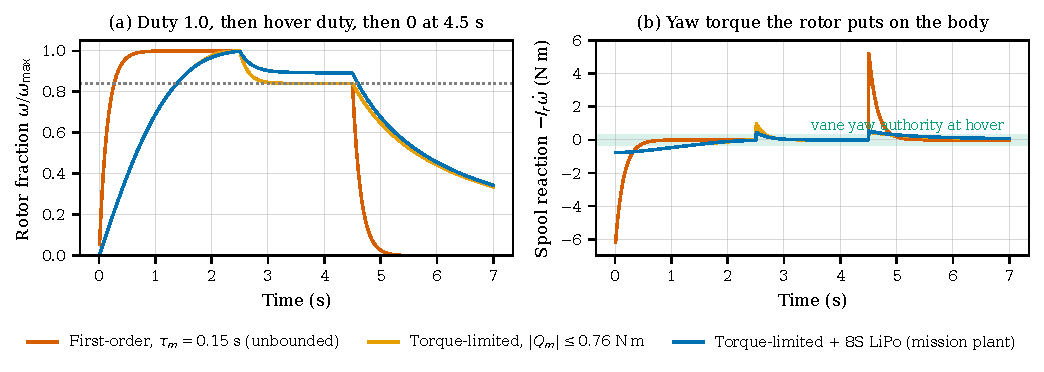
\includegraphics[width=0.92\textwidth]{spool.pdf}
\caption{Rotor response (a) and spool reaction torque on the body (b) for a cold spool-up at full duty, a step to hover duty and a cut to zero, at the \SI{120}{\hertz} mission step. The shaded band illustrates the vane-only moment scale at hover before the swirl reaction is included.}
\label{fig:spool}
\end{figure}

The pack is a one-branch Thevenin circuit~\cite{chen2006battery,plett2015} with open-circuit voltage $E(\mathrm{SOC})$, series resistance $R_0$ and polarization voltage $V_p$.
For a requested electrical power
\begin{equation}
P = \frac{1}{\eta_m}\left[Q_a\wrot + \frac{\mathrm{d}}{\mathrm{d}t}\!\left(\tfrac12\Ir\wrot^2\right)\right]^{+} + P_{\text{aux}},
\label{eq:power}
\end{equation}
the current is the high-voltage root of $\bar P = I(E' - IR_0)$ with $E' = E - V_p$, $I_{\lim} = \min(I_{\max},\, E'/(2R_0))$ and $\bar P = \min\!\left(P,\, I_{\lim}(E' - I_{\lim}R_0)\right)$,
\begin{equation}
I = \frac{2\bar P}{E' + \sqrt{E'^2 - 4R_0\bar P}}, \qquad I \le I_{\lim},
\label{eq:current}
\end{equation}
and $V = E' - IR_0$.
No regenerative charging is assumed.
Because the spool target depends on $V$ and the load depends on the spool, five damped fixed-point iterations resolve the pair at each substep.
When the pack cannot supply the request, the rotor may gain only the kinetic energy that the delivered shaft power provides:
\begin{equation}
\omega_r^{k+1} \le \sqrt{(\omega_r^{k})^2 + \frac{2\Delta t}{\Ir}\left(\eta_m(VI - P_{\text{aux}}) - Q_a\wrot\right)}.
\label{eq:energycap}
\end{equation}
At the initial level-hover speed fraction of 0.8409 the model draws \SI{2.085}{\kilo\watt}. In the \SI{5}{\ampere\hour} pack simulation the last logged sample within 0.01\% of that speed is at \SI{234}{\second}. The \SI{243}{\second} endpoint uses a 2\% speed-loss threshold. At the last sample the speed fraction is 0.8246, bus voltage is \SI{24.4}{\volt} and current is \SI{80}{\ampere}.
The thrust available to guidance therefore falls through a flight, which \refsec{sec:limits-derived} uses.

\subsection{Wake, Swirl and Rotor Reactions}
\label{sec:reactions}

The ideal jet speed scales with rotor speed, $u_{j,0} = u_{j,\max}\wrot/\wmax$, and the ideal wake power is $\tfrac12 T u_{j,0}$.
The stator does not recover all of the shaft torque.
The unrecovered part $Q_s = f_s P_{\max}(\wrot/\wmax)^3/\wrot$ leaves the nozzle as swirl, whose kinetic power must come out of the same shaft power:
\begin{equation}
\uj = \frac{u_{j,0}}{1 + Q_s^2/(T^2\langle r^2\rangle)}, \qquad \mdot = \frac{T}{\uj}, \qquad \Omega_s = \frac{Q_s}{\mdot\langle r^2\rangle},
\label{eq:wake}
\end{equation}
where $\langle r^2\rangle$ is the mean squared radius of the vane centers of pressure and $\Omega_s$ the swirl rate.
At hover $\mdot = \SI{0.316}{\kilogram\per\second}$ and $\uj = \SI{107.5}{\metre\per\second}$.

The rotor's angular momentum $\vect{H} = \Ir\wrot\ez$ is not part of the articulation, so its reactions are applied to the body explicitly and at full strength:
\begin{equation}
\vect{\tau}_{\text{spool}} = -\Ir\dot\omega_r\,\ez, \qquad
\vect{\tau}_{\text{swirl}} = -Q_s\,\ez, \qquad
\vect{\tau}_{\text{gyro}} = -\wb\times\vect{H}.
\label{eq:reactions}
\end{equation}
The swirl term equals and opposes the angular-momentum flux of the swirl the vanes then see, so the motor reaction, the stator recovery and the swirl close exactly; a unit test checks the closure to \num{1e-12}.

The scale of these reactions sets the vehicle's character and, in \refsec{sec:guidance}, the planner's rate bounds.
With $\Ir\wmax/I_{zz} = \SI{46.5}{\radian\per\second}$, a unit change in rotor fraction would spin the body by \SI{46.5}{\radian\per\second} if nothing resisted it, while the vanes supply \SI{0.35}{\newton\metre} at $+\SI{15}{\degree}$ before canceling the \SI{0.047}{\newton\metre} swirl reaction---a net yaw authority of $\pm\SI{0.30}{\newton\metre}$ at hover.
At hover $H = \SI{0.782}{\newton\metre\second}$, and the gyroscopic coupling $H/I_{xx} = \SI{15.6}{\radian\per\second}$ (\SI{2.49}{\hertz}) is the body's nutation frequency.
Spinning a cold rotor up in the air would hand the body about \SI{40}{\radian\per\second} of yaw, so missions start with the rotor at hover speed, which represents a spool-up on the pad.

\subsection{Jet-Vane Control-Volume Model}
\label{sec:vanes}

The original model treated each vane as an independent airfoil in the jet, $F_n = qSk_{\text{duct}}C_{N_\alpha}\alpha(1 - k_s\alpha^2)$ with $q = \tfrac12\rho \uj^2$.
At full rotor speed and \SI{15}{\degree} that law gives \SI{20.6}{\newton} of side force on one vane.
Under the assumptions of equal mass flow and a turn no larger than the vane angle at unchanged jet speed, a quarter of a \SI{48}{\newton} axial jet yields at most $(T/4)\sin\alpha = \SI{3.1}{\newton}$ of side force at \SI{15}{\degree}.
The airfoil law exceeds the momentum available by a factor of 6.6.

The replacement is a reduced-order control-volume model.
Four equal streamtubes share the mass flow $\mdot$ of \refeq{eq:wake}.
The velocity entering vane $i$, relative to the vane, is
\begin{equation}
\vect{v}_{\text{in},i} = \uj\,\ez + \Omega_s\ez\times\vect{r}_i^{\perp} + \wb\times\vect{r}_e - \dot{\vect{r}}_i ,
\label{eq:inflow}
\end{equation}
where $\vect{r}_i$ is the vane's measured, moving center of pressure, $\vect{r}_i^{\perp}$ its radial part, $\vect{r}_e$ the nozzle station and $\dot{\vect{r}}_i$ the center-of-pressure velocity relative to the body origin.
The terms follow a frozen convected wake: the jet leaves with its nozzle's velocity, and the vane moves through it.
With $\hat{\vect{N}}_i$ the zero-deflection vane normal, the deflected normal and chord are $\hat{\vect{n}}_i = \hat{\vect{N}}_i\cos\alpha_i - \ez\sin\alpha_i$ and $\hat{\vect{c}}_i = \hat{\vect{N}}_i\sin\alpha_i + \ez\cos\alpha_i$.
The vane removes a fraction $\tau_t$ of the velocity normal to its plane, then a fraction $\delta_D$ of the velocity along its chord:
\begin{gather}
\lambda = \frac{qSk_{\text{duct}}C_{N_\alpha}}{T/4}, \qquad
\lambda_D = \frac{qSk_{\text{duct}}C_{D_0}}{T/4}, \qquad
\tau_t = 1 - e^{-\lambda}, \qquad \delta_D = 1 - e^{-\lambda_D}, \nonumber\\
\vect{v}' = \vect{v}_{\text{in}} - \tau_t(\vect{v}_{\text{in}}\cdot\hat{\vect{n}})\hat{\vect{n}}, \qquad
\vect{v}_{\text{out}} = \vect{v}' - \delta_D(\vect{v}'\cdot\hat{\vect{c}})\hat{\vect{c}}.
\label{eq:turning}
\end{gather}
The exponential follows from integrating $\mathrm{d}v_n/\mathrm{d}x = -k v_n$ through the vane.
At small loading it recovers the thin-airfoil slope, and at high loading it aligns the flow with the vane instead of reversing it.
The force on each vane is the momentum change of its streamtube, applied at the vane's actual center of pressure:
\begin{equation}
\vect{F}_i = \frac{\mdot}{4}\left(\vect{v}_{\text{in},i} - \vect{v}_{\text{out},i}\right).
\label{eq:vaneforce}
\end{equation}

Three properties follow by construction and are covered by unit tests.
The vanes are passive, $\|\vect{v}_{\text{out}}\| \le \|\vect{v}_{\text{in}}\|$.
The body moment from the swirl reaction and the vanes equals the negative of the outgoing angular-momentum flux.
With no jet there is no force.
The axial component of $\sum_i\vect{F}_i$ is the vanes' thrust loss: \SI{4.93}{\newton}, or 10.3\% of static thrust, so the net static thrust is \SI{43.1}{\newton} and the net thrust-to-weight ratio is 1.41.
At zero deflection the vanes de-swirl the jet and cancel the \SI{0.047}{\newton\metre} residual swirl torque at hover to \SI{2.4e-5}{\newton\metre}.

\subsubsection{Closed Form in the Operating Regime}
\label{sec:closedform}

The loading $\lambda$ is independent of rotor speed, because $q$ and $T$ both scale with $\wrot^2$.
For the 8S parameters $\lambda = 7.61$, so $\tau_t = 0.9995$, and $\delta_D = 0.103$.
For a vane in an unswirled axial jet ($\Omega_s = 0$, $\wb = \vect{0}$, $\dot{\vect{r}}_i = \vect{0}$), \refeqs{eq:inflow}{eq:vaneforce} then reduce exactly to a side force of magnitude
\begin{equation}
F_{\perp} = \frac{T}{4}\left(\tau_t - \delta_D\right)\sin\alpha\cos\alpha ,
\label{eq:closed}
\end{equation}
directed against $\hat{\vect{N}}_i$.
The roll or pitch authority of an opposed vane pair with lever arm $\ell_z$ about the center of mass (for which first-order swirl effects cancel), and the yaw authority of a common-mode deflection at radius $r_v$, are therefore
\begin{equation}
\frac{\partial M_x}{\partial \alpha} = \frac{T}{2}(\tau_t - \delta_D)\,\ell_z, \qquad
\frac{\partial M_z}{\partial \alpha} = T(\tau_t - \delta_D)\,r_v .
\label{eq:authority}
\end{equation}
At hover ($T=\SI{33.9}{\newton}$, $\ell_z=\SI{0.11}{\metre}$, $r_v=\SI{0.04}{\metre}$) the full-model central difference at $\pm0.035$~rad gives roll and yaw slopes of 1.6725 and \SI{1.2163}{\newton\metre\per\radian}. At $\pm10^{-5}$~rad the slopes are 1.6738 and \SI{1.2173}{\newton\metre\per\radian}.
\reffig{fig:vanes} compares \refeq{eq:closed} with the model and the streamtube bound.

Equation~(\ref{eq:authority}) has two consequences for transfer to hardware.
First, the uncertain lift slope nearly drops out: $\partial\tau_t/\partial\ln C_{N_\alpha} = \lambda e^{-\lambda} \approx \num{4e-3}$, so halving $C_{N_\alpha}$ lowers the authority by 2.4\%.
What the authority does depend on is the assumption that each vane fully turns an equal quarter of the jet, together with the profile-drag fraction $\delta_D$.
Those, rather than $C_{N_\alpha}$, are what a thrust-stand vane sweep must identify.
Second, authority at hover is set by the vehicle's weight, not by the motor: the 6S and 8S profiles give the same hover authority to four digits.
The earlier model's small-angle roll authority is 8.47 times the present value throughout the modeled rotor-speed range. At full speed and \SI{15}{\degree}, the incremental side force from the coupled model is \SI{2.667}{\newton}, compared with \SI{2.691}{\newton} from the axial-flow expression. At fixed hover RPM, $+15^\circ$ common-mode deflection reduces net axial thrust from 30.45 to \SI{28.15}{\newton}.

\begin{figure}[t]
\centering
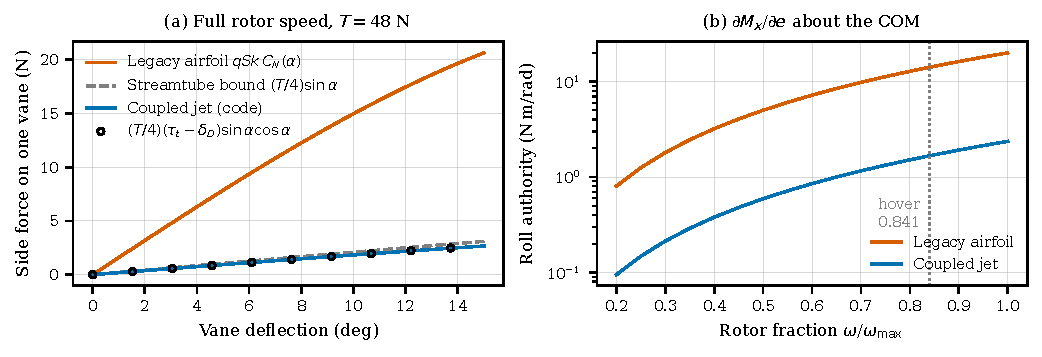
\includegraphics[width=0.92\textwidth]{vane_force.pdf}
\caption{(a) Side force on one vane at full rotor speed: the earlier independent-airfoil law, the streamtube bound $(T/4)\sin\alpha$, the coupled-jet model (with its $\alpha = 0$ de-swirl offset subtracted) and the closed form of \refeq{eq:closed}. (b) Roll authority about the center of mass against rotor fraction.}
\label{fig:vanes}
\end{figure}

\subsubsection{Actuation Chain}
\label{sec:servo}

The servo is a first-order lag with a slew limit and a deadband on the tracking error $\Delta = \alpha^{\text{cmd}} - \alpha_s$:
\begin{equation}
\alpha_s^{k+1} = \mathrm{clip}\!\left(\alpha_s^{k} + \Delta t\,\mathrm{clip}\!\left(\tfrac{e}{\tau_s}, \pm\dot\alpha_{\max}\right), \pm\alpha_{\max}\right), \qquad
e = \begin{cases}\Delta & |\Delta| \ge b,\\ 0 & \text{otherwise}.\end{cases}
\label{eq:servo}
\end{equation}
The servo can settle anywhere inside the error deadband. Mechanical backlash would additionally depend on the direction of travel and gear engagement.
The servo state is the target of an implicit joint drive whose overdamped response adds a lag of $c/k = \SI{25}{\milli\second}$.
The centers of pressure move with the vane links, and hinge moments from the aerodynamic load act on the drive through the engine.

\subsection{Intake Momentum Drag and Duct Jet Damping}
\label{sec:intake}

Static thrust $k_T\wrot^2$ counts only the momentum the jet leaves with.
The intake swallows $\mdot$ of air arriving at the vehicle's air-relative velocity and turns it onto the duct axis, which exerts the momentum drag familiar from ducted-fan vehicles~\cite{johnson2006ducted,pflimlin2010ducted}:
\begin{equation}
\vect{F}_{\text{in}} = -\mdot\left(\vect{v}_{\text{rel}} + \wb\times(\vect{r}_{\text{in}} - \vect{r}_c)\right),
\label{eq:intake}
\end{equation}
applied at the intake lip $\vect{r}_{\text{in}}$, which the asset geometry places \SI{0.007}{\metre} above the center of mass $\vect{r}_c$.
The force reads the same wind sample as the body drag, so gusts load the intake as well.
Body drag is quadratic in the air-relative velocity resolved in body axes, with separate axial and crossflow terms following the independence principle for slender bodies~\cite{hoerner1965}:
\begin{equation}
\vect{F}_{\perp} = -\tfrac12\rho C_{d,\perp}A_{\perp}\|\vect{v}_{\perp}\|\vect{v}_{\perp}, \qquad
F_{\parallel} = -\tfrac12\rho C_d A_{\parallel}|v_{\parallel}|v_{\parallel}.
\label{eq:bodydrag}
\end{equation}
Intake drag grows linearly with speed and body drag quadratically, so they are equal at $v = 2\mdot/(\rho C_{d,\perp}A_\perp) = \SI{12.3}{\metre\per\second}$ (\reffig{fig:drag}).
Below that speed the intake dominates: in a \SI{4}{\metre\per\second} wind it is \SI{1.26}{\newton}, 4\% of weight, against \SI{0.41}{\newton} of body drag.
The planner's point-mass model contains neither force; \refsec{sec:limits} returns to this.

\begin{figure}[t]
\centering
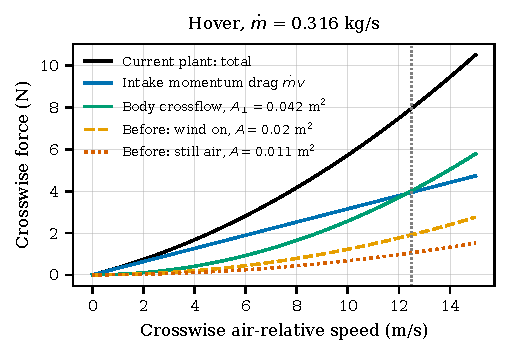
\includegraphics[width=0.52\textwidth]{drag.pdf}
\caption{Crosswise aerodynamic force at hover against air-relative speed. Intake momentum drag dominates below \SI{12.3}{\metre\per\second}. Dashed and dotted curves are the two body-drag paths of the earlier plant, neither of which included the intake.}
\label{fig:drag}
\end{figure}

The intake term is one half of the classical jet-damping bookkeeping.
Air crosses the duct from the inlet station $\vect{r}_i$ to the nozzle station $\vect{r}_e$ at a relative velocity $v_d\hat{\vect{a}}$, and a rotating vehicle must supply its Coriolis acceleration $2\wb\times v_d\hat{\vect{a}}$.
Integrating the reaction along the duct with $\mathrm{d}m = (\mdot/v_d)\,\mathrm{d}s$ gives
\begin{equation}
\vect{F}_{\text{cor}} = -2\mdot\,\wb\times(\vect{r}_e - \vect{r}_i), \quad \text{applied at } \tfrac12(\vect{r}_i + \vect{r}_e).
\label{eq:coriolis}
\end{equation}
For a duct on the body axis with stations $z_i$ and $z_e$ measured from the center of mass, its moment is $-\mdot(z_e^2 - z_i^2)\wb_\perp$.
Adding the intake moment $-\mdot z_i^2\wb_\perp$ gives $-\mdot z_e^2\wb_\perp$, the classical jet-damping moment, which depends only on the nozzle station~\cite{thomson1986}.
The pair is passive: with $\vect{v}$ the air-relative velocity of the center of mass, their total power is $-\mdot\|\vect{v} + \wb\times\vect{r}_e\|^2$.

\subsection{Passive Rotational Damping}
\label{sec:damping}

The original simulator applied a linear angular damper of \SI{0.27}{\newton\metre\second\per\radian} that had been tuned in simulation, with no physical source.
The mission plant removes it.
\reftab{tab:damping} quantifies what remains by perturbing the body rate at hover in the production code.
At a transverse rate of \SI{1}{\radian\per\second} the effective roll and pitch coefficient is \SI{2.07e-3}{\newton\metre\second\per\radian}, 131 times smaller than the removed damper. The yaw coefficient is \SI{5.05e-4}{\newton\metre\second\per\radian}.
The vane-flow term arises because body rotation enters \refeq{eq:inflow} and the vanes remove most of that relative flow.
The cylinder term is quadratic in rate. Omitting it in the small-amplitude limit gives $c=\SI{2.03e-3}{\newton\metre\second\per\radian}$ and a linearized nutation-amplitude decay rate $c/I_{xx}\simeq\SI{0.041}{\per\second}$.

\begin{table}[t]
\caption{Passive rotational damping at hover, from the production code (\si{\newton\metre\second\per\radian})}
\label{tab:damping}
\centering
\small
\begin{tabular}{lS[table-format=1.2e-1]S[table-format=1.2e-1]}
\toprule
Source & {Roll and pitch} & {Yaw} \\
\midrule
Earlier linear damper (removed) & 2.70e-1 & 2.70e-1 \\
\addlinespace
Cylinder crossflow drag at \SI{1}{\radian\per\second} & 3.45e-5 & {0} \\
Vane flow damping & 8.94e-4 & 5.05e-4 \\
Intake momentum drag, $\mdot z_i^2$ & 1.55e-5 & {0} \\
Duct Coriolis reaction, \refeq{eq:coriolis} & 1.12e-3 & {0} \\
Modeled total & 2.07e-3 & 5.05e-4 \\
\bottomrule
\end{tabular}
\end{table}

\subsection{Gyrostat Integration Inside a Rigid-Body Engine}
\label{sec:integration}

The engine integrates the locked-body Euler equation with an explicit treatment of $\wb\times\mat{I}\wb$, and a virtual rotor torque $-\wb\times\vect{H}$ evaluated at the old rate and applied as an external torque is also explicit.
Linearizing the torque-free gyrostat $\mat{I}\dot\wb + \wb\times(\mat{I}\wb + \vect{H}) = \vect{0}$ about a spin $r$ about the symmetry axis, the transverse rates rotate at the nutation frequency
\begin{equation}
\omega_n = \frac{\left|(I_{zz} - I_{xx})\,r + H\right|}{I_{xx}} ,
\label{eq:nutation}
\end{equation}
and an explicit Euler step multiplies the transverse kinetic energy by $1 + (\omega_n\Delta t)^2$ every step.
At hover with no body spin $\omega_n = \SI{15.6}{\radian\per\second}$; at \SI{120}{\hertz} the factor is 1.017 per step, which compounds to 57 in two seconds.
With initial transverse rates of \SI{6.28}{\radian\per\second} on each axis and \SI{40}{\radian\per\second} of counter-rotation, the ratio of final to initial \emph{body} kinetic energy, including the axial component, is \num{6.8e9} at \SI{120}{\hertz} and 76 at \SI{480}{\hertz}. The offline figure excludes rotor spin energy and the engine's angular-momentum projection.
A midpoint treatment of the rotor term alone does not help when the body term dominates.
Damping, or a reduced gyroscopic scale, would hide the error; neither is physical.

The mission plant therefore solves the body and rotor together with an implicit midpoint step,
\begin{equation}
\mat{I}(\wb_m - \wb_k) = \tfrac{\Delta t}{2}\left(\vect{\tau}_{\text{ext}} - \wb_m\times(\mat{I}\wb_m + \vect{H})\right), \qquad
\wb_{k+1} = 2\wb_m - \wb_k ,
\label{eq:midpoint}
\end{equation}
where $\vect{\tau}_{\text{ext}}$ collects the vane, spool, swirl, drag and intake moments about the center of mass and $\vect{H}$ uses the mean rotor speed over the step.
Four Newton iterations solve \refeq{eq:midpoint}.
The implicit midpoint rule conserves quadratic invariants, so for constant $\vect{H}$ and $\vect{\tau}_{\text{ext}} = \vect{0}$ it conserves both $\tfrac12\wb^\top\mat{I}\wb$ and $\|\mat{I}\wb + \vect{H}\|$~\cite{hairer2006}.
The engine still supplies its own explicit term $-\wb_k\times\mat{I}\wb_k$, so the environment applies the rotor torque together with an integration correction,
\begin{equation}
\vect{\tau}_{\text{gyro}} = \vect{H}\times\wb_m, \qquad
\vect{\tau}_{\text{corr}} = -\wb_m\times\mat{I}\wb_m + \wb_k\times\mat{I}\wb_k ,
\label{eq:correction}
\end{equation}
with which the engine's explicit step lands on the midpoint solution.
The correction is an integration bridge, not damping, and involves no target attitude.
Two details are needed for the bridge to hold.
After its explicit update the engine rescales the body's angular momentum to its pre-update magnitude, and the production mode inverts that projection in closed form.
The solver must also apply external forces once per step rather than at every iteration; the configuration loader rejects the coupled mode otherwise.

The engine advances orientation from the end-of-step rate, which is first order and inconsistent with the midpoint velocity.
In free flight the environment replaces it with the Lie-midpoint (Cayley) update paired with \refeq{eq:midpoint},
\begin{equation}
\vect{q}_{k+1} = \vect{q}_k\otimes\mathrm{normalize}\!\left(1,\; \tfrac{\Delta t}{4}\mat{D}(\wb_k + \wb_{k+1})\right),
\label{eq:cayley}
\end{equation}
which for constant $\vect{H}$ conserves world angular momentum as well as energy.
Whenever a contact is measured the engine's pose is left untouched, so contact impulses keep their exact effect.
\reffig{fig:gyro} shows both results in an offline replica of the integrator split.

\begin{figure}[t]
\centering
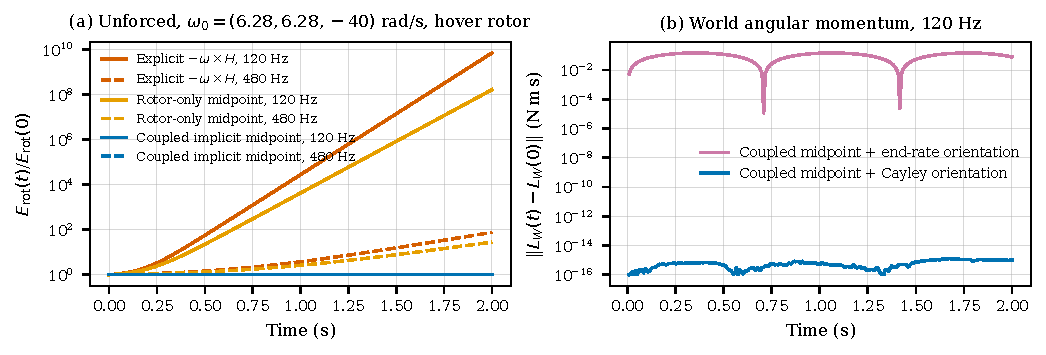
\includegraphics[width=0.92\textwidth]{gyro.pdf}
\caption{Offline replica of the integrator split for the unforced body and hover rotor, with body yaw counter to the rotor spin. (a) Rotational energy under an explicit gyroscopic torque, a rotor-only midpoint and the coupled midpoint of \refeq{eq:midpoint}, at \SI{120}{\hertz} (solid) and \SI{480}{\hertz} (dashed). (b) World angular-momentum error with an end-rate orientation update and with the Cayley update of \refeq{eq:cayley}.}
\label{fig:gyro}
\end{figure}

\subsection{Sensing, Contact and Success Criteria}
\label{sec:sensors}

The flight computer consumes the configured observation vector. The simulator can filter and delay navigation channels, while vane angles, vane rates and normalized rotor speed come directly from simulated states. Disabling sensor noise passes the original observations through.
An inertial measurement chain adds scale, misalignment, turn-on and Gauss--Markov biases, random walk, white noise and $g$-sensitivity to the true rate and specific force, then applies saturation, a first-order low-pass filter, quantization, sample-and-hold at the sensor's output rate and a transport delay; an onboard complementary filter produces attitude~\cite{mahony2008}.
An optional path fuses a rangefinder, an optical-flow sensor, a barometer and a pad fiducial in a 16-state error-state filter~\cite{sola2017,ardupilot2026ekf3}.
Latencies are rounded to whole physics substeps; each sensor model reports the rate and latency it actually delivers at the \SI{120}{\hertz} step, and a run warns when they differ from the datasheet by more than 25\%.

Landing detection uses contact reports on every link.
A four-state machine requires 15 consecutive contact frames before declaring a landing, records the largest downward speed at any first contact so a later gentle re-contact cannot hide a hard impact, and treats any vane contact as unsafe.
A landing counts as successful if the impact is at most \SI{0.25}{\metre\per\second} and the pad error at most \SI{0.5}{\metre}; an impact above \SI{3}{\metre\per\second}, a tilt above \SI{0.5}{\radian} at contact or an arrival rate above \SI{3}{\radian\per\second} is a crash.

\section{Convex Powered-Descent Guidance}
\label{sec:guidance}

\subsection{Problem Statement}
\label{sec:problem}

The planner treats the vehicle as a point mass with thrust acceleration $\vect{u} = \vect{T}/m$ in a world frame with $z$ up, $\vect{g} = (0, 0, -g)$.
The plan ends at a \emph{gate} $\vect{r}_g$ a fixed height above the touchdown point $\vect{a}$, descending vertically at $v_g$, from which a constant-rate terminal descent takes over.
The continuous-time problem is
\begin{subequations}
\label{eq:problem}
\begin{align}
\min_{t_f,\,\vect{u}(\cdot)}\quad & \int_0^{t_f} P\!\left(m\|\vect{u}(t)\|\right)\mathrm{d}t, \qquad P(T) = \frac{P_{\max}}{\eta_m}\left(\frac{T}{T_{\text{full}}}\right)^{3/2} + P_{\text{aux}}, \label{eq:prob-cost}\\
\text{subject to}\quad & \ddot{\vect{r}} = \vect{u} + \vect{g}, \qquad \vect{r}(0) = \vect{r}_0,\ \ \dot{\vect{r}}(0) = \vect{v}_0,\ \ \vect{u}(0) = \vect{u}_{\text{now}}, \label{eq:prob-dyn}\\
& \rho_1 \le m\|\vect{u}\| \le \rho_2, \qquad \ez\cdot\vect{u} \ge \|\vect{u}\|\cos\theta_{\max}, \label{eq:prob-annulus}\\
& \|\dot{\vect{u}}\| \le \dot T_{\max}/m, \qquad \|\dot{\vect{u}}_{xy}\| \le g\,\omega_t, \label{eq:prob-rate}\\
& \|\vect{v}\| \le \bar V(t), \qquad \|\vect{r}_{xy} - \vect{a}_{xy}\| \le \tan\gamma(t)\,(z - a_z), \label{eq:prob-state}\\
& z \ge z_g, \qquad -v_z \le \sqrt{v_g^2 + 2a\,(z - z_g)}, \label{eq:prob-sink}\\
& \vect{r}(t_f) = \vect{r}_g, \qquad \vect{v}(t_f) = (0, 0, -v_g), \qquad \vect{u}(t_f) = -\vect{g}. \label{eq:prob-term}
\end{align}
\end{subequations}
The thrust annulus in \refeq{eq:prob-annulus} is the only non-convex constraint; here $T_{\text{full}} = W / f_h^2 = \SI{43.07}{\newton}$ is the net static thrust at full rotor speed after the neutral vanes' axial drag loss.
Three features distinguish \refeq{eq:problem} from the rocket problem~\cite{acikmese2007}.
There is no mass dynamics, so no change of variables is needed and no approximation enters the thrust bounds.
The cost is a quasi-steady electrical-energy surrogate evaluated at neutral-vane net thrust. The plant also accounts for rotor kinetic-energy changes, dissipation during braking, voltage sag and vane deflection losses.
The rate constraints couple consecutive thrust vectors. Their initial value depends on whether the re-plan starts from a measurement or the preceding reference.

\subsection{Constraints Derived from the Plant}
\label{sec:limits-derived}

The model supplies thrust and torque scales. The reserve fractions and the speed, pointing and glide limits are design choices.
At every re-plan the flight computer derives them from a vehicle model that holds the mass, the level-hover rotor fraction $f_h$, the probed vane authorities $K = \SI{2.365}{\newton\metre\per\radian}$ and $K_{\psi} = \SI{1.720}{\newton\metre\per\radian}$ at full rotor speed, the rotor momentum $\Ir\wmax$, the inertias, the actuator lags, the nominal reference voltage $V_{\text{ref}} = \SI{29.6}{\volt}$ and the measured bus voltage $V$.
\reftab{tab:limits} lists the results.

\textit{Thrust annulus.}
The ceiling keeps half of the thrust above weight in reserve for the tracking loop,
\begin{equation}
\rho_2 = \max\!\left(1.01W,\, W + (1-r)(T_{\text{av}}(V)-W)\right), \quad r=0.5, \quad T_{\text{av}}(V)=T_{\text{full}}\min(1,V/V_{\text{ref}})^2 ,
\label{eq:rho2}
\end{equation}
and varies with the available thrust over the tested range of 26--\SI{33}{\volt}. At the endurance test's \SI{24.4}{\volt} endpoint, $T_{\text{av}}=\SI{29.26}{\newton}$ falls below the \SI{30.45}{\newton} weight. The numerical minimum gives $\rho_2=\SI{30.75}{\newton}$ there, so the planner can request thrust the vehicle cannot deliver.
The floor is positive for two reasons.
The vanes need jet flow for authority, so $\rho_1 \ge 0.6\,W$; and a plan may not accelerate downward harder than it can brake, $W - \rho_1 \le \rho_2 - W$.
The second condition is the active one on the 8S plant and sets $\rho_1 = 0.79\,W$.
Together the two bounds close the annulus symmetrically about weight as the battery discharges: at a \SI{26}{\volt} bus $T_{\text{av}} = \SI{33.2}{\newton}$ and the plan may use only \SIrange{29.1}{31.8}{\newton}.

\textit{Thrust rate.}
A duty slew $\dot d$ changes rotor speed at $\wmax(V/V_{\text{ref}})\dot d$, and the reaction torque about the thrust axis can be held only by the vanes' common mode.
The duty slew is bounded so that this reaction uses at most 40\% of the yaw torque available at hover,
\begin{equation}
\Ir\wmax\frac{V}{V_{\text{ref}}}\,\dot d \le 0.4\,\min\!\left(K_\psi f_h^2\bar\alpha,\ \tau_{\psi}\right),
\label{eq:dutyrate}
\end{equation}
with $\bar\alpha = \alpha_{\max} - b = \SI{0.245}{\radian}$ the vane effort limit (reserving the deadband $b$ inside the servo travel $\alpha_{\max}$) and $\tau_\psi = \SI{0.3}{\newton\metre}$ the yaw loop's design torque.
Through $T = T_{\text{full}}(d V/V_{\text{ref}})^2$ this becomes $\dot T_{\max} = 2\sqrt{T T_{\text{full}}}\,(V/V_{\text{ref}})\,\dot d$, evaluated conservatively at $T = 0.6\,W$.

\textit{Attitude slew.}
Tilting the body at a rate $\omega_t$ precesses the rotor and takes a vane torque $H\omega_t$.
The planned slew is limited to 40\% of the slew that usable vane deflection can sustain at hover,
\begin{equation}
\omega_t \le 0.4\,\frac{K f_h^2\bar\alpha}{\Ir\wmax f_h} ,
\label{eq:tiltrate}
\end{equation}
and the remaining torque is a design reserve for disturbance rejection.
The same expression with a 0.6 share bounds the body-rate command of the attitude loop.

\begin{table}[t]
\caption{Guidance limits derived from the 8S plant at a \SI{32}{\volt} bus}
\label{tab:limits}
\centering
\small
\begin{tabular}{lll}
\toprule
Quantity & Value & Origin \\
\midrule
Thrust floor $\rho_1$ & \SI{24.14}{\newton} (0.79\,$W$) & braking symmetry; at least $0.6\,W$ for vane authority \\
Weight $W$ & \SI{30.45}{\newton} & \\
Thrust ceiling $\rho_2$ & \SI{36.76}{\newton} (1.21\,$W$) & \refeq{eq:rho2}, $T_{\text{av}} = \SI{43.07}{\newton}$ \\
Duty slew & \SI{0.119}{\per\second} & \refeq{eq:dutyrate} \\
Thrust rate $\dot T_{\max}$ & \SI{7.19}{\newton\per\second} & duty slew at $0.6\,W$ \\
Horizontal slew scale $\omega_t$ & \SI{12.0}{\degree\per\second} & \refeq{eq:tiltrate} \\
Attitude-loop rate command & \SI{18.0}{\degree\per\second} & \refeq{eq:tiltrate} with share 0.6 \\
Emergency command rate & \SI{243}{\newton\per\second} & spool-up duty slew \SI{4}{\per\second} \\
Sink-envelope deceleration $a$ & \SI{0.71}{\metre\per\second\squared} & $0.35(\rho_2/m - g)$ \\
\addlinespace
Pointing $\theta_{\max}$, glide slope $\gamma$ & \SI{15}{\degree}, \SI{45}{\degree} & configuration \\
Speed bound & \SI{4}{\metre\per\second} & configuration \\
Gate & \SI{0.5}{\metre} above touchdown, \SI{0.15}{\metre\per\second} & configuration \\
\bottomrule
\end{tabular}
\end{table}

\subsection{Discretization}
\label{sec:discretization}

The thrust is a first-order hold: linear between $N + 1$ nodes rather than piecewise constant.
The dynamics are integrated exactly over each interval of length $\Delta t = t_f/N$,
\begin{equation}
\begin{split}
\vect{r}_{k+1} &= \vect{r}_k + \Delta t\,\vect{v}_k + \Delta t^2\left(\tfrac13\vect{u}_k + \tfrac16\vect{u}_{k+1} + \tfrac12\vect{g}\right),\\
\vect{v}_{k+1} &= \vect{v}_k + \Delta t\left(\tfrac12(\vect{u}_k + \vect{u}_{k+1}) + \vect{g}\right),
\end{split}
\label{eq:foh}
\end{equation}
and the tracking loop samples the plan exactly, as a cubic in position.
A measured-start plan uses the rotor speed and body axis, projecting the initial thrust onto the admissible pointing cone and limiting its magnitude to available thrust. An ordinary reference-start re-plan uses the preceding plan's thrust. The floor and ceiling can ramp from an initially out-of-band magnitude.
Because the planned thrust is continuous, a bound on its node-to-node change bounds the thrust the vehicle has to follow.
A zero-order hold stepped the thrust direction at every node: on a recorded \SI{30}{\metre} approach those steps reached \SI{8.6}{\degree} every \SI{0.46}{\second}, which the rate-limited rotor and the precession-limited attitude loop cannot follow.
The landing leg uses $N = 24$.

\subsection{Lossless Convexification and a Gap Guard}
\label{sec:lcvx}

Following A\c{c}{\i}kme\c{s}e and Ploen~\cite{acikmese2007}, the annulus is relaxed with a slack $\sigma_k$,
\begin{equation}
\|\vect{u}_k\| \le \sigma_k, \qquad \rho_1/m \le \sigma_k \le \rho_2/m, \qquad u_{z,k} \ge \sigma_k\cos\theta_{\max},
\label{eq:lcvx}
\end{equation}
and the cost is written on $\sigma$.
For the classical problem the relaxation is lossless: at the optimum $\|\vect{u}_k\| = \sigma_k$, so the planned thrust respects the annulus~\cite{acikmese2007,acikmese2011lcvx}.
Problem~(\ref{eq:problem}) leaves the hypotheses of that result in two ways.
The rate bounds of \refeq{eq:prob-rate} couple successive controls, and state constraints are known to break the guarantee in general~\cite{harris2014lcvx}.
The simultaneous state, endpoint and rate constraints preclude attributing a measured gap to a particular constraint from an active-set observation alone.
We therefore treat losslessness as a property to be measured.
Every plan reports the gap
\begin{equation}
\epsilon = \max_k\,\frac{\sigma_k - \|\vect{u}_k\|}{\sigma_k},
\label{eq:gap}
\end{equation}
and \refsec{sec:results-planner} shows that it is not always zero.

When a fixed-duration solve returns $\epsilon > \num{e-3}$, the nodes whose own gap exceeds the tolerance receive a convex half-space floor along their solved unit thrust direction $\hat{\vect{d}}_k$,
\begin{equation}
\vect{u}_k\cdot\hat{\vect{d}}_k \ge \min\!\left(\rho_{1}/m,\ \|\vect{u}_{\text{now}}\| + (\dot T_{\max}/m)\,t_k\right),
\label{eq:floor}
\end{equation}
which by Cauchy--Schwarz implies $\|\vect{u}_k\| \ge \rho_1/m$ (after any initial spool-up ramp) and acts as a single selective successive-convexification step on the concave floor, and the problem is solved once more.
The added inequality enforces the floor at the selected node. The re-solve can move other nodes, and a chord between two admissible thrust vectors can pass inside the excluded ball.
In the duration search a plan whose residual gap still exceeds \num{e-3} counts as infeasible and is returned only if no duration yields a tight plan.
Plans that were already tight never trigger the guard and are unchanged by it.

\subsection{Discrete Constraints}
\label{sec:constraints}

All constraints are convex and imposed at the nodes.
\begin{itemize}
\item \textit{Thrust rate.} $\|\vect{u}_{k+1} - \vect{u}_k\| \le \dot T_{\max}\Delta t/m$ on the thrust vector. A bound on the slack would not bound $\|\vect{u}\|$ once $\sigma > \|\vect{u}\|$; the vector form also bounds the direction slew.
\item \textit{Attitude slew.} $\|\vect{u}_{xy,k+1} - \vect{u}_{xy,k}\| \le g\,\omega_t\Delta t$, which bounds the tilt rate to first order in tilt for a vertical thrust component near $g$.
\item \textit{Glide slope.} $\|\vect{r}_{xy,k} - \vect{a}_{xy}\| \le \tan\gamma_k\,(z_k - a_z)$. A start outside the \SI{45}{\degree} cone gets a cone widened to contain it that narrows linearly back to nominal \SI{3}{\second} before the gate; the half-angle of each node is fixed before the solve, so the constraint stays a second-order cone.
\item \textit{Speed.} $\|\vect{v}_k\| \le \max\!\left(V_{\max},\ v_e - b_v\,(t_k - t_s)^+\right)$. A fast entry keeps its speed $v_e$ while the rate-limited thrust settles over $t_s$, then brakes back under $V_{\max}$ at half the slowest braking the limits allow. A single cap based on $\|\vect{v}_0\|$ let each re-plan fly faster than the last.
\item \textit{Sink-rate envelope.} The last constraint of \refeq{eq:prob-sink} is imposed through an auxiliary $s_k$ with $-v_{z,k} \le s_k + r_k$ and the rotated second-order cone $\|(2s_k,\, L_k - 1)\| \le L_k + 1$, $L_k = v_g^2 + 2a(z_k - z_g)$, where $r_k \ge 0$ is an entry braking slack (zero unless the start already sinks faster than the envelope after thrust settling, in which case it decays to zero at the full planned braking acceleration). The envelope uses instantaneous upright acceleration $a=0.35(\rho_2/m-g)$. At \SI{26}{\volt} this is \SI{0.157}{\metre\per\second\squared}, while the reserved thrust at \SI{15}{\degree} tilt supplies only \SI{0.098}{\metre\per\second\squared} vertically above gravity. Returning upright takes time. In an earlier run without the envelope the plan braked on the thrust-rate bound, which is the whole yaw-safe duty slew, and left the tracking loop no slew to make up the rotor's lag.
\item \textit{Gate.} \refeq{eq:prob-term} at node $N$, and $z_k \ge z_g$ on the landing leg. The final thrust is vertical and equals weight, so the hand-over to the terminal descent needs no thrust step.
\item \textit{Routes.} A fly-through waypoint constrains a node to a capture ball and its velocity to the leg speed along the route tangent, or to a cone around it; a hover waypoint fixes position, zero velocity and hover thrust. An optional soft corridor prices the distance of each node from a chord of the drawn route beyond a half-width.
\end{itemize}

\subsection{Objective}
\label{sec:objective}

Each node gets an epigraph variable $c_k \ge \sigma_k^{3/2}$, expressed as the power cone $(c_k, 1, \sigma_k) \in \mathcal{K}_{\text{pow}}(2/3)$, and the nodes are combined with trapezoid weights $w_k$:
\begin{equation}
\min\ \sum_{k=0}^{N} w_k c_k + J_{\text{sec}}, \qquad c_k^{2/3}\cdot 1^{1/3} \ge \sigma_k .
\label{eq:energy}
\end{equation}
The auxiliary power is constant per unit time and is added when durations are compared.
A propulsive velocity-increment objective $\sum_k w_k\sigma_k$, the analogue of the original fuel cost, is the alternative.
The optional secondary terms $J_{\text{sec}}$---cross-track distance from a drawn route, duration, squared thrust jerk and squared horizontal thrust---are priced in seconds of hover cost and make the problem a quadratic-objective conic program.
None involves $\sigma$.
All are zero in the repository defaults under which the reported missions flew.

\subsection{Free Final Time and Fallback}
\label{sec:freetime}

For a fixed duration the planner sends Clarabel a convex program with second-order and power cones, 24 intervals and about 300 variables.
The duration is found by a one-dimensional search over such problems, as in the original method.
Without a previous plan, the search samples eight durations geometrically between bounds set by distance and the speed limit; when re-planning it samples three around the previous plan's remaining time.
Six golden-section steps follow~\cite{kiefer1953}.
Independent durations are solved in parallel on four threads.
Problems are solved with Clarabel~0.11~\cite{goulart2024clarabel} with a \SI{0.5}{\second} wall-time limit per conic solve.

If the duration search finds no hard-terminal solution, a soft-terminal problem minimizes a weighted gate-position and velocity miss.
The fallback relaxes the state and terminal requirements, penalizes ground-clearance shortfall, and permits full available thrust and the emergency command slew.
The emergency command rate in \reftab{tab:limits} is a duty-derived allowance. At hover $Q_a=\SI{0.467}{\newton\metre}$, and the motor torque cap gives $2T_{\text{full}}f_h(\bar Q-Q_a)/(\Ir\wmax)=\SI{22.8}{\newton\per\second}$ of upward net-thrust slew before further pack limits.

\section{Flight Control}
\label{sec:control}

\subsection{Closed-Loop Execution and Tracking}
\label{sec:closedloop}

The flight computer re-solves every \SI{0.5}{\second}, when the route changes, or when the tracking error exceeds \SI{0.75}{\metre}.
While the vehicle tracks within \SI{0.75}{\metre} and \SI{0.75}{\metre\per\second} of the plan, the new plan starts from the old plan's reference state, so feedback keeps acting on the deviation; re-solving from the measured state every period zeroed the tracking error each time and, in a recorded mission, let the vehicle orbit the pad.
Larger deviations re-plan from the measured state.
Re-planning stops \SI{0.8}{\second} before the gate.
A deployment model makes planning latency explicit: a re-plan requested at time $t$ replaces the tracked plan only at $t + t_{\text{plan}}$, with its clock starting at $t$, and on the flight computer the solve runs in a separate process beside the \SI{30}{\hertz} loop.
A braking monitor integrates the fastest stop the yaw-safe duty slew allows; if that stop needs more than 85\% of the height above touchdown, the duty slews at the spool-up rate instead, trading a yaw transient for braking.

The plan's thrust acceleration, sampled one spool lag ahead and linearly cross-faded over \SI{0.3}{\second} across re-plans to suppress slope-change kicks, is the feedforward, and world-frame feedback corrects it:
\begin{equation}
\vect{a}_{\text{cmd}} = \vect{u}_{\text{ff}}(t + t_{\text{lead}}) + \mat{K}_p\vect{e}_r + \mat{K}_d\vect{e}_v + \mat{K}_i\!\int\mathrm{sat}(\vect{e}_r)\,\mathrm{d}t .
\label{eq:track}
\end{equation}
The integrators accumulate only near steady flight ($\|\vect{u}_{\text{ff}} + \vect{g}\| \le \SI{1.0}{\metre\per\second\squared}$) so maneuver lag does not wind them up, and absorb thrust-model bias, wind and the side force of a center-of-mass trim; this is the only path by which the aerodynamic forces of \refsec{sec:intake} reach the guidance.
The direction of $m\vect{a}_{\text{cmd}}$ is the desired body axis, and its component along the actual body axis sets the duty by inverting the battery-coupled speed law, $d = \sqrt{T/T_{\text{full}}}\,V_{\text{ref}}/V$, at the measured bus voltage.
The duty slew of \refeq{eq:dutyrate} is applied to the rotor command $dV/V_{\text{ref}}$ rather than to the raw duty, so a duty change that only compensates a bus-voltage change passes at once.

The lateral loop has a subtlety specific to jet vanes.
The vanes push the vehicle sideways directly, at $Kf_h^2/(\ell_z m) \approx \SI{4.9}{\metre\per\second\squared}$ per radian of effort at hover, and that push opposes the tilt they command, which makes the lateral response non-minimum-phase.
A linear hover model of the complete loop shows that this side force caps the usable velocity gain.

\subsection{Gyroscopic Attitude Regulation}
\label{sec:lqr}

The attitude error is geometric, $\vect{e} = \tfrac12(\mat{R}_d^\top\mat{R} - \mat{R}^\top\mat{R}_d)^\vee$~\cite{lee2010geometric}, with the heading left free.
The rotor's momentum dominates roll and pitch:
\begin{equation}
\begin{split}
I\dot p &= Kf^2 j_x - Hq - cp, \qquad I\dot q = Kf^2 j_y + Hp - cq,\\
\dot s &= (u_c - s)/\tau_s, \qquad\quad \dot j = (s - j)/\tau_j ,
\end{split}
\label{eq:attplant}
\end{equation}
where $H = \Ir\wmax f$, $u_c$ is the commanded effort, $s$ the servo angle and $j$ the vane-joint angle in effort space, with $\tau_s = \SI{0.05}{\second}$ and $\tau_j = \SI{25}{\milli\second}$.
The torque-free transverse mode has angular frequency $H/I$ or cyclic frequency $H/(2\pi I)\simeq\SI{2.49}{\hertz}$ at hover.
At that frequency the servo and joint lags contribute about \SI{59}{\degree} of phase lag together. A half-sample delay at \SI{30}{\hertz} contributes another \SI{15}{\degree}. The closed-loop eigenvalues below include the sampled actuator dynamics.

The regulator is a discrete linear-quadratic design on the full state of \refeq{eq:attplant}, $\vect{x} = [\int\!\vect{e},\, \vect{e},\, \wb_{xy} - \wb_{\text{ref}},\, \vect{s} - \vect{s}_h,\, \vect{j} - \vect{j}_h]$, ten states for roll and pitch.
The simulation supplies $j$ and $\dot j$. Under the assumed joint lag the regulator reconstructs $s=j+\tau_j\dot j$. Equivalent hardware feedback remains to be established.
The gains solve the discrete algebraic Riccati equation for the zero-order-hold model at \SI{30}{\hertz}, with the input weighted by Bryson's rule on vane torque~\cite{bryson1975} so that the design is the same torque loop on any vanes, and are scheduled on rotor fraction because both $Kf^2$ and $H$ change with it.
Yaw is a separate channel whose integral cancels the residual-swirl torque.
To follow a turning plan the regulator tracks a rate reference bounded by the planned slew, with vane offsets that sustain the corresponding precession.
The mixer gives roll and pitch priority except for a common-mode reserve that holds the rotor reaction at the bounded duty slew.
Each vane command is pre-compensated for the servo deadband with a backlash inverse~\cite{tao1996}, $\alpha^{\text{cmd}} = \alpha_{\text{des}} + b\,\mathrm{sat}((\alpha_{\text{des}} - s)/(0.25\,b))$.

\section{Results}
\label{sec:results}

\subsection{Plant Verification}
\label{sec:results-plant}

The plant is verified in three layers.
The first is a suite of unit tests on the tensor models: frames, vane geometry, the servo, the motor and battery, the coupled jet's conservation and passivity, rotor reactions, the gyroscopic midpoint, wind and intake drag, the contact state machine, the sensor and navigation models, and the controller and planner.
For this paper the suite was run on a CPU-only machine; 437 tests passed and two that need the asset's geometry bindings were skipped.
The offline experiments reproduce the predicted small-angle authority and the torque-free midpoint invariants. In the counter-rotating case of \reffig{fig:gyro}, the explicit update amplifies body kinetic energy by \num{6.8e9}, while the coupled midpoint/Cayley update preserves body kinetic energy and world angular momentum to round-off.
The third layer is the project's recorded open-loop audit of the plant in the rigid-body engine, with scripted vanes and duty and no controller (\reftab{tab:audit}).
Nutation frequency, steady precession under a vane step, yaw acceleration and the momentum exchange of a throttle cut agree with first-principles predictions to within about 5\% at both \SI{120}{\hertz} and \SI{480}{\hertz}.
That audit preceded the intake and duct terms of \refsec{sec:intake}, and its nutation decay of 0.018--\SI{0.019}{\per\second} matches the vane-flow coefficient of \reftab{tab:damping} alone, $c/I_{xx} = \SI{0.018}{\per\second}$.

\begin{table}[t]
\caption{Open-loop audit of the momentum-vane plant in the rigid-body engine (recorded)}
\label{tab:audit}
\centering
\small
\begin{tabular}{llll}
\toprule
Test & \SI{120}{\hertz} & \SI{480}{\hertz} & Prediction \\
\midrule
Nutation frequency, neutral vanes & \SI{2.489}{\hertz} & \SI{2.492}{\hertz} & $H/(2\pi I_{xx}) = \SI{2.49}{\hertz}$ \\
Nutation decay rate & \SI{0.019}{\per\second} & \SI{0.018}{\per\second} & \SI{0.018}{\per\second} \\
Roll step, steady precession & \SI{3.70}{\degree\per\second} & \SI{3.72}{\degree\per\second} & \SI{3.9}{\degree\per\second} \\
Yaw step, common mode & \SI{110.6}{\degree\per\second\squared} & \SI{111.1}{\degree\per\second\squared} & \SI{114}{\degree\per\second\squared} \\
Throttle cut in the air & \SI{2242}{\degree\per\second} & \SI{2242}{\degree\per\second} & $\Delta H/I_{zz} = \SI{2233}{\degree\per\second}$ \\
\bottomrule
\end{tabular}
\end{table}

\subsection{Planner Behavior}
\label{sec:results-planner}

\subsubsection{A Representative Plan}

\reffig{fig:plan} shows the reference plan from $(8, 5, 18)$~\si{\metre} at rest with the limits of \reftab{tab:limits}.
The plan lasts \SI{8.54}{\second} and costs \SI{4.97}{\watt\hour} in the quasi-steady surrogate.
It reaches \SI{6.2}{\degree} tilt. The maximum horizontal thrust-acceleration rate divided by $g$ is \SI{11.33}{\degree\per\second}, and the actual unit-thrust-direction rate peaks at \SI{10.44}{\degree\per\second}.
Its thrust rate reaches the bound during the initial ramp-down, and the relaxation is tight, $\epsilon = \num{1.7e-9}$.
One artifact is visible in panel (b): while the envelope binds, the planned thrust alternates by about \SI{\pm0.5}{\newton} from node to node, because the constraints hold only at the nodes and the first-order hold lets alternating thrusts satisfy them there.
The rotor's rate limit filters the alternation, and the smoothness term of \refsec{sec:objective} removes it.

\begin{figure}[t]
\centering
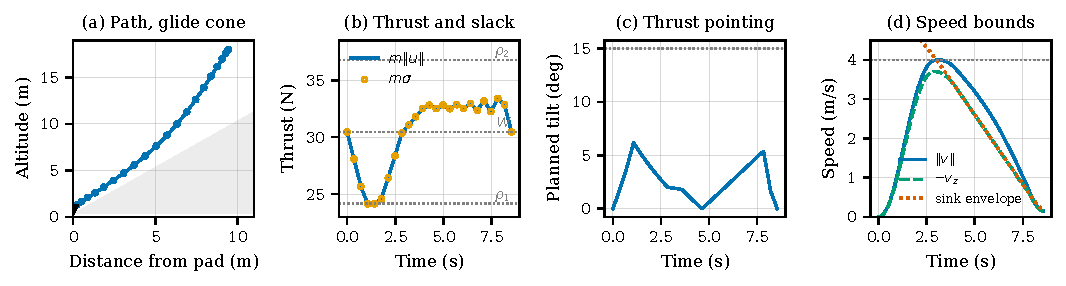
\includegraphics[width=\textwidth]{convex_plan.pdf}
\caption{Reference plan from $(8, 5, 18)$ m at rest. (a) Horizontal distance against altitude; the shaded region is excluded by the \SI{45}{\degree} glide cone and the triangle marks the gate. (b) Planned thrust $m\|\vect{u}\|$ and slack $m\sigma$ at the nodes, with $\rho_1$, $W$ and $\rho_2$. (c) Planned tilt. (d) Speed against its bound, and sink rate against the envelope.}
\label{fig:plan}
\end{figure}

\subsubsection{Dispersed Starts}

To characterize the planner beyond single cases, 400 starts were drawn uniformly: horizontal offset 0--\SI{25}{\metre} at a random azimuth, altitude 5--\SI{40}{\metre}, horizontal speed 0--\SI{3}{\metre\per\second} in a random direction, vertical speed between \SI{-3}{} and \SI{+1}{\metre\per\second}, and a bus voltage of 26--\SI{33}{\volt}, with the limits re-derived at each voltage and the rotor at hover thrust.
Each start was planned once without a previous plan, on an Apple M1 Max.
\reftab{tab:mc} and \reffig{fig:mc} summarize the outcome.

A plan was returned for every start.
The search returned 355 hard-terminal plans (89\%).
The other 45 switched to soft-terminal plans with gate-position and velocity residuals below $10^{-8}$ in SI units. Keeping the hard constraints and checking durations from 3 to \SI{35.75}{\second} at \SI{0.25}{\second} intervals recovered a hard-terminal plan for zero-based case 336 at \SI{17.75}{\second} ($\epsilon=\num{2.3e-9}$). A fallback records a search outcome.
Among the 355 hard-terminal results, planning took a median of \SI{62}{\milli\second}, \SI{90}{\milli\second} at the 95th percentile and \SI{117}{\milli\second} at worst. The median search used 15 conic solves. Across all 400 requests in the same run, the median and 95th percentile were 63 and \SI{94}{\milli\second}, respectively.
For comparison the project measured \SI{48}{\milli\second} mean per landing plan on a desktop processor and estimates that the embedded computers under consideration are four to five times slower, which places a landing re-plan at 0.2--\SI{0.4}{\second} against the \SI{0.5}{\second} re-plan period.

\begin{table}[t]
\caption{Planner outcome over 400 dispersed starts (production planner, $N = 24$, energy objective)}
\label{tab:mc}
\centering
\small
\begin{tabular}{lcc}
\toprule
 & Relaxation as solved & With gap guard \\
\midrule
Hard-terminal / soft-terminal / no plan & 355 / 45 / 0 & 355 / 45 / 0 \\
Gap $\epsilon$, median over hard-terminal plans & \num{3.2e-9} & \num{2.8e-9} \\
Gap $\epsilon$, maximum & \num{3.4e-2} & \num{6.3e-4} \\
Hard-terminal plans with $\epsilon > \num{e-3}$ & 72 (20\%) & 0 \\
Energy change on those 72 plans, median / maximum & --- & $+2.0\%$ / $+10.3\%$ \\
Duration change on those 72 plans, median / maximum & --- & $+\SI{0.29}{\second}$ / $+\SI{1.43}{\second}$ \\
Hard-terminal wall time, median / 95th percentile / maximum & 61 / 86 / \SI{95}{\milli\second} & 62 / 90 / \SI{117}{\milli\second} \\
Conic solves per hard-terminal plan, median / maximum & 15 / 15 & 15 / 18 \\
\bottomrule
\end{tabular}
\end{table}

\begin{figure}[t]
\centering
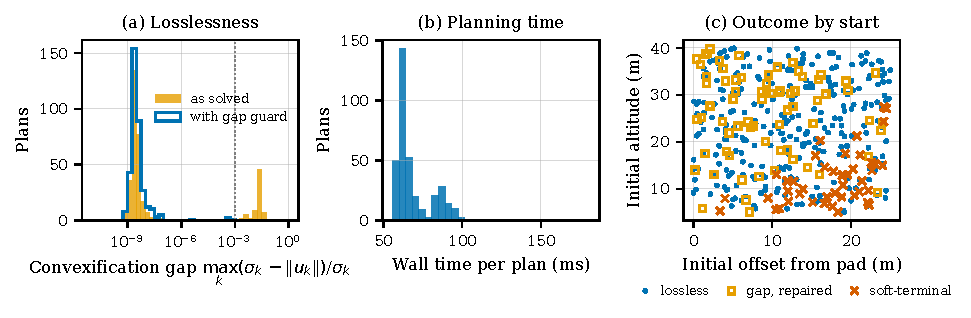
\includegraphics[width=\textwidth]{planner_mc.pdf}
\caption{Planner outcome over 400 dispersed starts. (a) Node gap of the hard-terminal plans as solved and with the gap guard; the dotted line is the tolerance. (b) Wall time for the 355 hard-terminal plans. (c) Outcome against the start's offset and altitude.}
\label{fig:mc}
\end{figure}

\subsubsection{Tightness of the Relaxation}

The relaxation is tight to solver precision for most starts, but not for all.
As solved, 72 of the 355 hard-terminal plans (20\%) have a gap above \num{e-3}, up to 3.4\%; the gap distribution is bimodal, with nothing between \num{e-6} and \num{e-3} (\reffig{fig:mc}a).
The gapped starts are steeper than the rest, with a median ratio of offset to altitude of 0.32 against 0.55 for all starts.
In the gapped plans the low-thrust nodes occurred during the descent ramp.
Early in the plan, while thrust ramps down at the rate bound to shed altitude quickly, one to six nodes (one at the median) place $\|\vect{u}\|$ below $\sigma = \rho_1/m$: the planned thrust dips under the floor while the slack stays on it.
In every gapped node the slack is on its lower bound.
The violation is small in absolute terms, a median of \SI{0.65}{\newton} and at most \SI{0.97}{\newton} below the floor, and the lowest planned thrust of \SI{23.4}{\newton} remains well above the \SI{18.3}{\newton} authority floor because $\rho_1$ is set here by braking symmetry.
At the same durations, removing only the full-vector rate inequality left 47 of the 72 above $\epsilon=10^{-3}$, with a maximum gap of 3.41\%. The horizontal slew and state constraints were retained in the formulation. The pointing cone itself gives $\epsilon\le 1-\cos\theta_{\max}=3.4074\%$.
With the guard of \refsec{sec:lcvx} no hard-terminal plan has a gap above \num{6.3e-4}.
The repaired plans are longer by a median of \SI{0.29}{\second} and cost a median of 2.0\% more energy, with a worst case of 10.3\%; plans that were already tight are unchanged.

We checked the guarded solutions along every first-order-hold interval. For $\vect{u}(s)=\vect{u}_0+s\Delta\vect{u}$, $0\le s\le1$, the minimum norm occurs at $s_*=\mathrm{clip}(-\vect{u}_0\cdot\Delta\vect{u}/\|\Delta\vect{u}\|^2,0,1)$ for nonconstant thrust. The unit-direction rate is $\|\vect{u}_0\times\Delta\vect{u}\|/(\Delta t\,\|\vect{u}(s)\|^2)$, so its maximum occurs at the same point.
Across 355 guarded hard-terminal plans, 121 crossed below the floor by more than \SI{e-5}{\newton}. The largest shortfall was \SI{0.1253}{\newton} in case 301, whose node gap was below \num{4e-8}. In 131 plans the direction rate exceeded the configured horizontal slew scale of \SI{12.01}{\degree\per\second}. Case 229 reached \SI{16.35}{\degree\per\second}.

\subsubsection{Structure of the Free-Final-Time Problem}

\reffig{fig:search} shows the cost of the fixed-duration problem against duration for the plan of \reffig{fig:plan} and for ten of the dispersed starts.
Planned energy grows nearly linearly across the solved duration samples, at about \SI{0.58}{\watt\hour\per\second}.

With the gap guard disabled, the first 60 dispersed starts were solved on a \SI{0.5}{\second} grid from 2 to \SI{30}{\second}.
For the 53 with a solution, solved samples were contiguous and cost was non-decreasing from the first solved sample. Fitted slopes ranged from 0.577 to \SI{0.579}{\watt\hour\per\second}.

This slope agrees with the modeled hover power of \SI{2.085}{\kilo\watt}.
In the reference case the normal search returned \SI{8.544}{\second} and \SI{4.9668}{\watt\hour}. The first solved point on the original \SI{0.25}{\second} grid was \SI{8.50}{\second}.
Refining the sampling to \SI{0.01}{\second} yielded a hard-terminal solution at \SI{8.45}{\second}, with $\epsilon<\num{5e-8}$ and cost \SI{4.9201}{\watt\hour}.
The search result therefore costs 0.95\% more than this candidate alone.
The grids resolve a trend over sampled durations. Locating the shortest feasible duration or the global minimum would require a separate bound.


\begin{figure}[t]
\centering
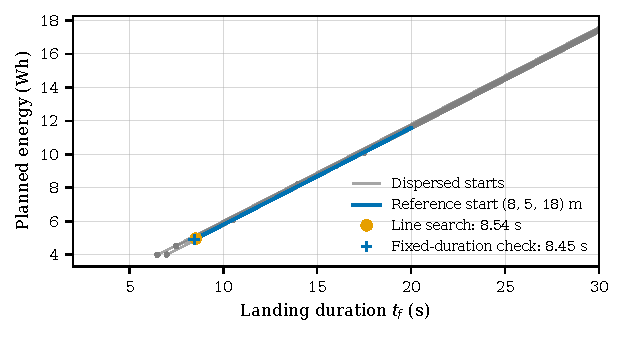
\includegraphics[width=0.62\textwidth]{duration_search.pdf}
\caption{Planned energy at solved duration samples for the reference start and ten dispersed starts. Curves begin at their first solved sample. The circle marks the normal search result. The cross marks the additional fixed-duration check.}
\label{fig:search}
\end{figure}

\subsubsection{Discretization}

\reffig{fig:nodes} varies the number of landing-leg intervals for the plan of \reffig{fig:plan}.
At the production value $N = 24$ the planned energy is within 0.03\% of the $N = 96$ value.
The constraints hold only at the nodes, and dense sampling of the first-order-hold plan shows by how much they are exceeded in between: at $N = 24$ the sink-rate envelope is exceeded by at most \SI{0.016}{\metre\per\second} and the speed bound by \SI{0.002}{\metre\per\second}, and the planned thrust falls at most \SI{0.001}{\newton} below $\rho_1$ on the chord between two nodes.
Below $N = 16$ the excess grows to several centimetres per second.
In this run planning took \SI{94}{\milli\second} at $N=24$ and \SI{327}{\milli\second} at $N=96$. Each resolution was timed once.

\begin{figure}[t]
\centering
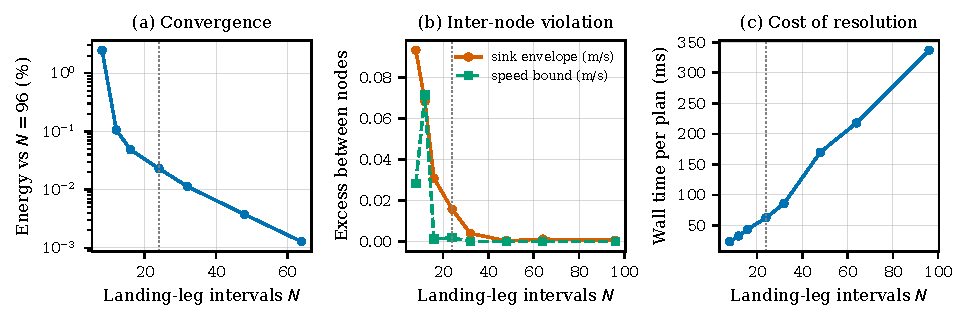
\includegraphics[width=\textwidth]{planner_nodes.pdf}
\caption{Effect of the number of landing-leg intervals $N$ on the plan of \reffig{fig:plan}. (a) Planned energy relative to $N = 96$. (b) Largest excess over the sink-rate envelope and the speed bound between nodes. (c) Wall time per plan. The dotted line marks the production value $N = 24$.}
\label{fig:nodes}
\end{figure}

\subsection{Attitude Stability on the Corrected Plant}
\label{sec:results-attitude}

\reffig{fig:lqr} compares the growth rate of the slowest closed-loop roll and pitch mode of \refeq{eq:attplant} under the earlier proportional-derivative law and under the scheduled regulator.
On the momentum-vane plant the earlier law is linearly unstable above a rotor fraction of 0.67, which covers the whole flight range: at hover it has a \SI{4.1}{\hertz} mode growing at \SI{1.68}{\per\second} and a \SI{1.6}{\hertz} mode growing at \SI{1.05}{\per\second}.
On the earlier plant the \SI{0.27}{\newton\metre\second\per\radian} damper had masked this instability, and on the corrected plant only saturation and the servo deadband bounded it, as the limit cycles observed in the recorded runs.
The regulator's slowest modes at hover decay at 1.92 and \SI{3.96}{\per\second}, and the smallest damping ratio among modes above \SI{0.5}{\hertz} is 0.46 at hover and 0.40 over the range.
The project's robustness checks keep that ratio at or above 0.24 under $\pm30\%$ authority, $+50\%$ actuator lag, \SI{8}{\milli\second} of extra delay, $\pm20\%$ inertia or $+20\%$ rotor momentum, applied one at a time.
The modeled servo deadband had sustained a \SI{1}{\hertz} coning limit cycle at \SI{15}{\degree\per\second} of body-rate RMS in every recorded mission; in an offline replica the backlash inverse reduced it to \SI{1.2}{\degree\per\second}.

\begin{figure}[t]
\centering
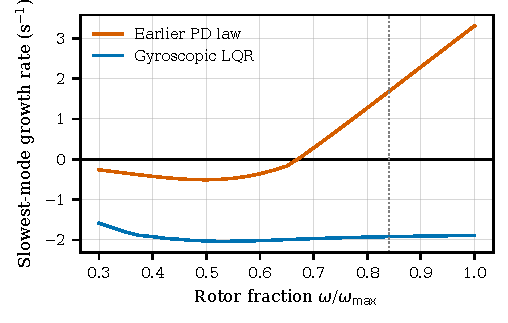
\includegraphics[width=0.5\textwidth]{lqr.pdf}
\caption{Growth rate of the slowest closed-loop roll and pitch mode on the attitude model of \refeq{eq:attplant} at the \SI{30}{\hertz} control period, against rotor fraction. The dotted line marks hover.}
\label{fig:lqr}
\end{figure}

\subsection{Dispersed Closed-Loop Landings on a Reduced-Order Replica}
\label{sec:results-closedloop}

The recorded missions of \refsec{sec:results-missions} are few.
To assess closed-loop behavior over the dispersed starts of \refsec{sec:results-planner}, the production flight computer---planner, tracking loop, attitude regulator, mixer and deadband inverse, unmodified and built from the plant as the mission runner builds it---was flown on a reduced-order replica of the plant.
The replica extends the one used by the project's unit tests.
The replica treats the rotor gyroscopic term by implicit midpoint at \SI{120}{\hertz}, advances the locked-body Euler term explicitly, and updates orientation using the rotation exponential. Its angular model omits duct and vane-flow damping.
Vane torques act at the probed authorities $K$ and $K_\psi$ scaled by $f^2$, together with the side force those torques imply at the vane lever arm, so the non-minimum-phase lateral path is present.
The servo is the production model with its deadband, followed by the \SI{25}{\milli\second} joint lag.
The motor is the current-limited model of \refeq{eq:esc} and \refeq{eq:motor} on a constant bus voltage.
A steady wind acts through intake momentum drag and body drag.
The replica omits contact (a run ends when the body reaches touchdown height), the sensor chain (the controller reads the true state), battery sag within a flight, gusts and the coupled-jet model itself.
It is therefore a test of the guidance and control logic under dispersion, not of the plant model, and its landing statistics are optimistic with respect to sensing and contact.

The 400 starts are those of \reftab{tab:mc}, each with its bus voltage and with a steady wind of 0--\SI{4}{\metre\per\second} in a random direction.
All 400 runs crossed the body-origin touchdown-height threshold within the specified pad and downward-speed tolerances (\reffig{fig:closedloop}).
At that crossing the median and maximum downward speeds were 0.152 and \SI{0.206}{\metre\per\second}, and the median and maximum total body speeds were 0.177 and \SI{0.228}{\metre\per\second}. The median and maximum pad errors were 0.101 and \SI{0.333}{\metre}. First-leg contact velocity also depends on attitude, angular velocity and foot location.
The 46 runs that at some point tracked a soft-terminal plan, among them the 45 whose first plan was one, landed like the rest.
All 111 runs in the 26--\SI{28}{\volt} group passed the crossing criteria, with median downward speed \SI{0.153}{\metre\per\second}.
The peak tilt in flight grows with the initial offset and reaches \SI{19}{\degree}; it exceeds the \SI{15}{\degree} planning cone in 22 runs and stays inside the tracking loop's \SI{22}{\degree} limit.
The roll and pitch rate RMS has a median of \SI{2.9}{\degree\per\second}.

\reftab{tab:variants} repeats the first 100 starts with one change at a time; in the mismatch cases the controller is unchanged and unaware of the change.
With the earlier proportional-derivative attitude law every run still lands, but the roll and pitch rate RMS rises from 2.8 to \SI{12.2}{\degree\per\second} (\reffig{fig:closedloop}c).
The earlier law has locally unstable modes in the linear model. The nonlinear simulations exhibit bounded oscillations with the actuator limits and servo deadband active.
All 100 cases with a fixed \SI{0.4}{\second} re-plan delay still met the crossing criteria. This imposed delay tests tracking and does not measure embedded solve time.
A rotor inertia 20\% above the controller's model and a \SI{5}{\milli\metre} lateral center-of-mass offset are also tolerated; the offset raises the median tilt at touchdown from 1.4 to \SI{2.7}{\degree}.
Vanes 30\% weaker than modeled are not fully tolerated.
Ninety-three runs passed. Two crossed 1.4 and \SI{1.7}{\metre} from the pad, and five timed out after \SI{120}{\second}.
The 30\% authority reduction produced the largest loss of completions among the perturbations tested. Its speed and pad summaries include the 95 runs that reached the crossing.

\begin{figure}[t]
\centering
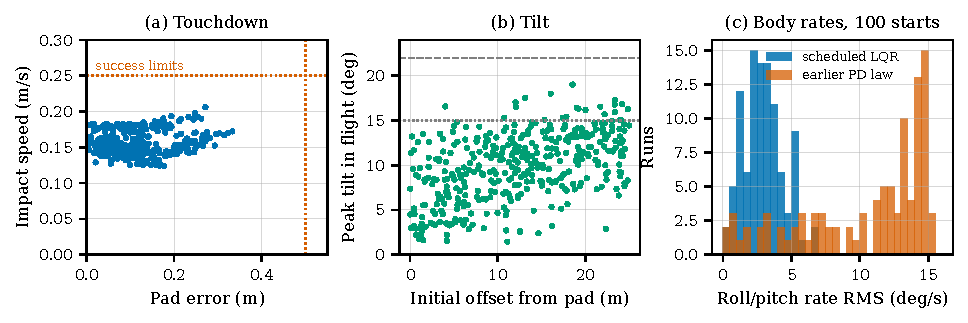
\includegraphics[width=\textwidth]{closed_loop.pdf}
\caption{Closed-loop landings on the reduced-order replica. (a) Downward body speed at the height crossing against pad error for the 400 dispersed starts, with the success limits. (b) Peak tilt in flight against the initial offset; the dotted and dashed lines are the planning cone and the tracking loop's limit. (c) Roll and pitch rate RMS over the first 100 starts with the scheduled regulator and with the earlier proportional-derivative law.}
\label{fig:closedloop}
\end{figure}

\begin{table}[t]
\caption{Closed-loop landings on the reduced-order replica: the first 100 dispersed starts, one change at a time (rate RMS and tilt at touchdown are medians)}
\label{tab:variants}
\centering
\small
\begin{tabular}{lccccc}
\toprule
Case & Passed & Downward speed, \si{\metre\per\second} & Pad error, \si{\metre} & Rate RMS, & Final tilt, \\
 & of 100 & median / max & median / max & \si{\degree\per\second} & \si{\degree} \\
\midrule
Production controller, nominal plant & 100 & 0.153 / 0.187 & 0.110 / 0.293 & 2.8 & 1.4 \\
Earlier proportional-derivative law & 100 & 0.153 / 0.204 & 0.098 / 0.266 & 12.2 & 2.3 \\
Planning latency \SI{0.4}{\second} & 100 & 0.153 / 0.189 & 0.116 / 0.297 & 3.1 & 1.4 \\
Plant rotor inertia $+20\%$ & 100 & 0.154 / 0.189 & 0.106 / 0.282 & 2.8 & 1.4 \\
Center-of-mass offset \SI{5}{\milli\metre} & 100 & 0.149 / 0.194 & 0.082 / 0.289 & 3.2 & 2.7 \\
Plant vane authority $-30\%$ & 93 & 0.151 / 0.189 & 0.123 / 1.696 & 3.4 & 1.4 \\
\bottomrule
\end{tabular}
\end{table}

\subsection{Recorded Missions in the Rigid-Body Engine}
\label{sec:results-missions}

\reftab{tab:missions} summarizes eight earlier rigid-body missions on the momentum-vane plant, each starting with the rotor at hover speed.
All eight landed inside the success criteria of \refsec{sec:sensors}, with impacts of 0.136--\SI{0.178}{\metre\per\second} and pad errors of 0.004--\SI{0.146}{\metre}.
Two later re-flights on the plant with intake momentum drag also landed: a high-energy capture at \SI{0.142}{\metre\per\second} and \SI{0.204}{\metre}, and a gust station-keeping mission at \SI{0.128}{\metre\per\second} and \SI{0.116}{\metre}.
With the intake force the vehicle leans \SI{5.5}{\degree} into a \SI{4}{\metre\per\second} wind and holds station within \SI{0.40}{\metre}; without it the wind barely reached the vehicle.

Two kinds of mission fail for physical reasons that the simulator reproduces.
Cold in-air starts fail because spooling the rotor moves \SI{0.78}{\newton\metre\second} into a body whose vanes hold about \SI{0.3}{\newton\metre} in yaw.
A \SI{1}{\centi\metre} lateral center-of-mass offset fails because trimming it needs about \SI{10}{\degree} of the vanes' \SI{14}{\degree} usable travel; the replica (\refsec{sec:results-closedloop}) tolerated half that offset.

The eight September 26 missions preceded the September 28 sink-rate envelope and braking emergency, the corrected intake station, duct Coriolis reaction and node-gap guard. They demonstrate the earlier controller and plant combination.
The wind-lean result also used the earlier intake lever arm of \SI{0.10}{\metre}, compared with \SI{0.007}{\metre} in the present model.
At hover the added duct damping of \SI{1.12e-3}{\newton\metre\second\per\radian} exceeds the modeled vane-flow roll damping of \SI{8.94e-4}{\newton\metre\second\per\radian}.
A re-flight tool restores each recorded mission from its request, flies it on the current plant and reports every outcome and dynamics setting that differs.
A read-only replay of the project's mission-control console, with 13 recorded flights of this guidance in the rigid-body engine, two of them failures, can be viewed at \url{https://triaggent.com/portfolio/mission-control/}.

\begin{table}[t]
\caption{Recorded closed-loop missions, convex guidance on the momentum-vane plant}
\label{tab:missions}
\centering
\small
\begin{tabular}{lccc}
\toprule
Mission & Impact, \si{\metre\per\second} & Pad error, \si{\metre} & Roll/pitch rate RMS, flight / terminal, \si{\degree\per\second} \\
\midrule
Default descent from \SI{18}{\metre} & 0.178 & 0.017 & 0.7 / 0.8 \\
Hop, \SI{3}{\metre} & 0.154 & 0.045 & 5.6 / 3.9 \\
\SI{7}{\metre} offset with crosswind & 0.159 & 0.052 & 6.8 / 2.7 \\
Legacy 6S pack, \SI{8}{\metre} & 0.175 & 0.051 & 7.3 / 1.4 \\
Start at \SI{50}{\metre} & 0.152 & 0.004 & 0.7 / 0.7 \\
Route with fly-through and hover & 0.152 & 0.098 & 7.3 / 3.3 \\
\SI{50}{\metre}, three hovers, \SI{120}{\second} & 0.148 & 0.063 & 3.8 / 3.2 \\
Wind, sensor noise, mass offset, \SI{-5}{\metre\per\second} entry & 0.136 & 0.146 & 9.3 / 4.6 \\
\bottomrule
\end{tabular}
\end{table}

\section{Limitations and Identification Plan}
\label{sec:limits}

\textit{Jet-speed convention.}
The plant takes the nozzle jet speed from $\sqrt{2T/\rho A}$ with the fan's swept area $A = \SI{4780}{\milli\metre\squared}$, which is the far-wake speed of an open rotor.
At \SI{48}{\newton}, a pressure-matched uniform jet at \SI{128}{\metre\per\second} requires an effective area of \SI{2390}{\milli\metre\squared}. Taking the exit area equal to the full swept area instead gives $\sqrt{T/(\rho A)}=\SI{90.5}{\metre\per\second}$. Exit pressure and velocity profiles remain unmeasured.
The reference shaft power of \SI{3072}{\watt} then corresponds to a fan efficiency of 0.71 rather than to an ideal jet, which is plausible.
Rebuilding the production models with the ducted speed raises the hover mass flow by 38\%, from 0.316 to \SI{0.434}{\kilogram\per\second}, and with it the intake drag (\SI{1.74}{\newton} instead of \SI{1.26}{\newton} at \SI{4}{\metre\per\second}) and the jet damping.
It halves the vane loading to $\lambda = 3.8$ and the vanes' axial loss to 5.3\%, and raises the vane authority by only 3\%, as \refeq{eq:authority} predicts.
At unchanged shaft-power reference, the alternate convention increases full-speed net thrust by 5.6\% and lowers modeled hover electrical power from 2.085 to \SI{1.924}{\kilo\watt}. The sensitivity test recalculates plant parameters only.
The exit area should be measured and the jet speed confirmed with a pitot traverse.

\textit{Vane model.}
The authority of \refeq{eq:authority} rests on equal streamtube shares and almost complete turning.
Real vanes may not intercept a full quarter of the jet each, and hub blockage, wall proximity and vane-to-vane interference are absent.
The radial vane span is 0.019--\SI{0.047}{\metre}. Its geometric centroid at \SI{0.033}{\metre} is 17.5\% inboard of the assumed \SI{0.040}{\metre} pressure radius. The force distribution determines the actual moment arm.
The identification target is the normalized side force $F_\perp/(T/4)$ against $\alpha$, together with $\delta_D$, measured on a thrust stand.

\textit{Planner model.}
The point-mass model contains no aerodynamics.
With prescribed mass flow, intake drag is affine in air-relative velocity. Using the plant's thrust-dependent mass flow introduces a product with velocity.
The horizontal slew proxy assumes a vertical thrust component near $g$. The interval checks in \refsec{sec:results-planner} quantify the discrepancy throughout the dispersed plans.
The guard supplies a one-pass repair of selected node floors. A continuous trajectory feasibility guarantee would require independent checks of the inter-node path and state constraints.
A wall-time limit can interrupt a solve under processor contention, leaving a feasible duration unrecognized.
Planning latency on the target computer, estimated at 0.2--\SI{0.4}{\second} for a landing plan and several seconds for a long route, has been exercised only on the replica of \refsec{sec:results-closedloop}, for landing plans.

\textit{Environment and actuators.}
Gusts are horizontal steps. The upright nozzle sits \SI{0.7625}{\metre} above the pad at the gate and \SI{0.2625}{\metre} at touchdown, approximately 8.5 and 2.9 fan diameters. The model omits ground effect and pad impingement.
The axial intake term is a first-order thrust lapse.
Whether the speed controller brakes actively during a throttle reduction is firmware-dependent.
The rotor inertia, which scales every momentum effect and therefore the thrust-rate and attitude-slew bounds, is an estimate, as are the servo lag and deadband and all battery coefficients.
Sensor latencies are rounded to the \SI{8.3}{\milli\second} physics substep.

\textit{Evidence.}
All closed-loop results are simulated.
The dispersed campaign uses a reduced-order replica with no contact, no sensor chain, no deflection-induced axial thrust loss and no in-flight battery sag (a \SI{26}{\volt} loaded 8S bus already sits near 4\% state of charge, where dynamic polarization sag during braking can trip a \SI{24}{\volt} pack cutoff), so it bounds neither touchdown dynamics, estimation error nor deep-discharge cutoff.
The missions in the rigid-body engine are few, and they predate the latest plant corrections and the gap guard.

The open parameters group into a short list of bench experiments:
a thrust stand, static and at airspeed, for $T(\wrot, V)$, $P(\wrot)$, the jet speed, the inflow thrust lapse and the vane sweep;
an independent rotor-inertia measurement and coast-down data to identify $Q_a/\Ir$, followed by a loaded spool step response;
a loaded servo response for the lag, slew, deadband and drive stiffness;
a pack discharge at hover power for the battery circuit;
a static inertial log for an Allan-variance fit;
and a bifilar swing for the inertia tensor together with a free-flight nutation test, whose frequency and decay (\SI{2.49}{\hertz} and \SI{0.041}{\per\second} modeled) check the rotor momentum, the inertia and the passive damping at once.

\section{Conclusion}
\label{sec:conclusion}

For the modeled jet-vane EDF, rotor angular momentum limits the available slew authority, and the loaded bus voltage determines how much thrust is available above weight.
We described a plant model that is bounded by momentum and energy bookkeeping, and a guidance law that takes its constraints from that model.
Three findings bear on the use of convex guidance for such vehicles.
The node-gap guard reduced the largest hard-terminal gap below $10^{-3}$. Exact first-order-hold checks still found small inter-node thrust-floor violations.
Across the sampled solved durations, planned energy rose at approximately the hover power. Finer duration checks recovered solutions missed by the initial search.
And the fidelity of the plant decides the control problem: the momentum bound on the vanes and the removal of an artificial damper made the previous attitude law unstable and required a regulator that feeds back the actuator states.
All 400 nominal replica runs met the touchdown-height crossing criteria. Reducing vane authority by 30\% produced seven off-pad crossings or timeouts in 100 matched starts. Hardware validation remains open.
Two lines of work follow.
The first is a comparison of geometric integrators for the body--rotor gyrostat on energy conservation and stability, setting the schemes examined here against other structure-preserving schemes across step sizes and spin rates.
The second, and the more important, is to build the vehicle and test how well the model and the guidance transfer to it: the thrust-stand and bench measurements of \refsec{sec:limits} identify the plant, the recorded missions are re-flown on the identified plant together with a dispersed campaign in the rigid-body engine, and the simulated landings are compared with flight.

\section*{Appendix: Reproducibility}

The figure scripts import the simulator's model classes and load the mission configuration; none requires the rigid-body engine.
Scripts under \texttt{Paper/physics\_simulation/scripts} produce Figs.~\ref{fig:spool}--\ref{fig:plan} and \ref{fig:lqr} and print the numbers quoted in Sections~\ref{sec:plant} and \ref{sec:results-attitude}; for this draft each was re-run and its printed output compared with the stored output.
\texttt{Paper/aiaa\_conference/scripts/fig\_planner\_study.py} produces Figs.~\ref{fig:mc}--\ref{fig:nodes}, \reftab{tab:mc} and the duration-structure statistics from a fixed random seed, \texttt{sens\_jet\_speed.py} produces the jet-speed sensitivity of \refsec{sec:limits}, and \texttt{fig\_closed\_loop.py} flies the closed-loop campaign of \refsec{sec:results-closedloop} and its variants and produces \reffig{fig:closedloop} and \reftab{tab:variants}.
Printed outputs are stored beside the figures.
The scripts need PyTorch, NumPy, SciPy, PyYAML, Matplotlib and Clarabel.
Timings were measured on an Apple M1 Max with four solver threads.

\setlength{\bibsep}{1pt}
\begin{thebibliography}{99}

\bibitem{acikmese2007}
A\c{c}{\i}kme\c{s}e, B., and Ploen, S. R., ``Convex Programming Approach to Powered Descent Guidance for Mars Landing,'' \textit{Journal of Guidance, Control, and Dynamics}, Vol.~30, No.~5, 2007, pp.~1353--1366.

\bibitem{acikmese2013lcvx}
A\c{c}{\i}kme\c{s}e, B., Carson, J. M., and Blackmore, L., ``Lossless Convexification of Nonconvex Control Bound and Pointing Constraints of the Soft Landing Optimal Control Problem,'' \textit{IEEE Transactions on Control Systems Technology}, Vol.~21, No.~6, 2013, pp.~2104--2113.

\bibitem{blackmore2016}
Blackmore, L., ``Autonomous Precision Landing of Space Rockets,'' \textit{The Bridge}, Vol.~46, No.~4, National Academy of Engineering, 2016, pp.~15--20.

\bibitem{scharf2017}
Scharf, D. P., A\c{c}{\i}kme\c{s}e, B., Dueri, D., Benito, J., and Casoliva, J., ``Implementation and Experimental Demonstration of Onboard Powered-Descent Guidance,'' \textit{Journal of Guidance, Control, and Dynamics}, Vol.~40, No.~2, 2017, pp.~213--229.

\bibitem{linsen2022}
Linsen, R., Listov, P., de Lajarte, A., Schwan, R., and Jones, C. N., ``Optimal Thrust Vector Control of an Electric Small-Scale Rocket Prototype,'' \textit{Proceedings of the IEEE International Conference on Robotics and Automation (ICRA)}, 2022, pp.~1996--2002.

\bibitem{furrer2016rotors}
Furrer, F., Burri, M., Achtelik, M., and Siegwart, R., ``RotorS---A Modular Gazebo MAV Simulator Framework,'' \textit{Robot Operating System (ROS): The Complete Reference (Volume 1)}, edited by A. Koubaa, Springer, Cham, 2016, pp.~595--625.

\bibitem{song2020flightmare}
Song, Y., Naji, S., Kaufmann, E., Loquercio, A., and Scaramuzza, D., ``Flightmare: A Flexible Quadrotor Simulator,'' \textit{Proceedings of the Conference on Robot Learning (CoRL)}, 2020.

\bibitem{shah2018airsim}
Shah, S., Dey, D., Lovett, C., and Kapoor, A., ``AirSim: High-Fidelity Visual and Physical Simulation for Autonomous Vehicles,'' \textit{Field and Service Robotics}, Springer, Cham, 2018, pp.~621--635.

\bibitem{panerati2021gym}
Panerati, J., Zheng, H., Zhou, S., Xu, J., Prorok, A., and Schoellig, A. P., ``Learning to Fly---A Gym Environment with PyBullet Physics for Reinforcement Learning of Multi-Agent Quadcopter Control,'' \textit{Proceedings of the IEEE/RSJ International Conference on Intelligent Robots and Systems (IROS)}, 2021.

\bibitem{acikmese2011lcvx}
A\c{c}{\i}kme\c{s}e, B., and Blackmore, L., ``Lossless Convexification of a Class of Optimal Control Problems with Non-Convex Control Constraints,'' \textit{Automatica}, Vol.~47, No.~2, 2011, pp.~341--347.

\bibitem{harris2014lcvx}
Harris, M. W., and A\c{c}{\i}kme\c{s}e, B., ``Lossless Convexification of Non-Convex Optimal Control Problems for State Constrained Linear Systems,'' \textit{Automatica}, Vol.~50, No.~9, 2014, pp.~2304--2311.

\bibitem{blackmore2010mle}
Blackmore, L., A\c{c}{\i}kme\c{s}e, B., and Scharf, D. P., ``Minimum-Landing-Error Powered-Descent Guidance for Mars Landing Using Convex Optimization,'' \textit{Journal of Guidance, Control, and Dynamics}, Vol.~33, No.~4, 2010, pp.~1161--1171.

\bibitem{dueri2017}
Dueri, D., A\c{c}{\i}kme\c{s}e, B., Scharf, D. P., and Harris, M. W., ``Customized Real-Time Interior-Point Methods for Onboard Powered-Descent Guidance,'' \textit{Journal of Guidance, Control, and Dynamics}, Vol.~40, No.~2, 2017, pp.~197--212.

\bibitem{szmuk2018}
Szmuk, M., and A\c{c}{\i}kme\c{s}e, B., ``Successive Convexification for 6-DoF Mars Rocket Powered Landing with Free-Final-Time,'' \textit{2018 AIAA Guidance, Navigation, and Control Conference}, AIAA Paper 2018-0617, 2018.

\bibitem{malyuta2022convex}
Malyuta, D., Reynolds, T. P., Szmuk, M., Lew, T., Bonalli, R., Pavone, M., and A\c{c}{\i}kme\c{s}e, B., ``Convex Optimization for Trajectory Generation: A Tutorial on Generating Dynamically Feasible Trajectories Reliably and Efficiently,'' \textit{IEEE Control Systems Magazine}, Vol.~42, No.~5, 2022, pp.~40--113.

\bibitem{goulart2024clarabel}
Goulart, P. J., and Chen, Y., ``Clarabel: An Interior-Point Solver for Conic Programs with Quadratic Objectives,'' \textit{Mathematical Programming Computation}, Vol.~18, 2026, pp.~1279--1361.

\bibitem{sutton2017}
Sutton, G. P., and Biblarz, O., \textit{Rocket Propulsion Elements}, 9th ed., Wiley, Hoboken, NJ, 2017.

\bibitem{sung2004jetvane}
Sung, H.-G., and Hwang, Y.-S., ``Thrust-Vector Characteristics of Jet Vanes Arranged in X-Formation Within a Shroud,'' \textit{Journal of Propulsion and Power}, Vol.~20, No.~3, 2004, pp.~501--508.

\bibitem{liu2013jetvane}
Liu, F., and Wang, L., ``Research on the Thrust Vector Control via Jet Vane in Rapid Turning of Vertical Launch,'' \textit{Proceedings of the 2nd International Conference on Measurement, Information and Control (ICMIC)}, IEEE, Harbin, China, 2013, pp.~837--842.

\bibitem{johnson2006ducted}
Johnson, E. N., and Turbe, M. A., ``Modeling, Control, and Flight Testing of a Small Ducted-Fan Aircraft,'' \textit{Journal of Guidance, Control, and Dynamics}, Vol.~29, No.~4, 2006, pp.~769--779.

\bibitem{pflimlin2010ducted}
Pflimlin, J.-M., Binetti, P., Sou\`eres, P., Hamel, T., and Trouchet, D., ``Modeling and Attitude Control Analysis of a Ducted-Fan Micro Aerial Vehicle,'' \textit{Control Engineering Practice}, Vol.~18, No.~3, 2010, pp.~209--218.

\bibitem{drela2006qprop}
Drela, M., ``QPROP Formulation,'' Massachusetts Institute of Technology, Department of Aeronautics and Astronautics, Cambridge, MA, 2006.

\bibitem{thomson1986}
Thomson, W. T., \textit{Introduction to Space Dynamics}, Dover, New York, 1986.

\bibitem{makoviychuk2021isaac}
Makoviychuk, V., Wawrzyniak, L., Guo, Y., Lu, M., Storey, K., Macklin, M., Hoeller, D., Rudin, N., Allshire, A., Handa, A., and State, G., ``Isaac Gym: High Performance GPU-Based Physics Simulation for Robot Learning,'' \textit{Proceedings of the NeurIPS Datasets and Benchmarks Track}, 2021.

\bibitem{mittal2023orbit}
Mittal, M., Yu, C., Yu, Q., Liu, J., Rudin, N., Hoeller, D., Yuan, J. L., Tehrani, P. P., Singh, R., Guo, Y., Mazhar, H., Mandlekar, A., Babich, B., State, G., Hutter, M., and Garg, A., ``Orbit: A Unified Simulation Framework for Interactive Robot Learning Environments,'' \textit{IEEE Robotics and Automation Letters}, Vol.~8, No.~6, 2023, pp.~3740--3747.

\bibitem{simo1991}
Simo, J. C., and Wong, K. K., ``Unconditionally Stable Algorithms for Rigid Body Dynamics That Exactly Preserve Energy and Momentum,'' \textit{International Journal for Numerical Methods in Engineering}, Vol.~31, No.~1, 1991, pp.~19--52.

\bibitem{hairer2006}
Hairer, E., Lubich, C., and Wanner, G., \textit{Geometric Numerical Integration}, 2nd ed., Springer, Berlin, 2006.

\bibitem{lee2007lie}
Lee, T., Leok, M., and McClamroch, N. H., ``Lie Group Variational Integrators for the Full Body Problem,'' \textit{Computer Methods in Applied Mechanics and Engineering}, Vol.~196, 2007, pp.~2907--2924.

\bibitem{physx2023}
NVIDIA Corporation, ``PhysX SDK 5 Documentation: Articulations,'' 2023.

\bibitem{lee2010geometric}
Lee, T., Leok, M., and McClamroch, N. H., ``Geometric Tracking Control of a Quadrotor UAV on SE(3),'' \textit{Proceedings of the IEEE Conference on Decision and Control}, 2010, pp.~5420--5425.

\bibitem{bryson1975}
Bryson, A. E., and Ho, Y.-C., \textit{Applied Optimal Control}, Hemisphere, Washington, DC, 1975.

\bibitem{tao1996}
Tao, G., and Kokotovi\'c, P. V., \textit{Adaptive Control of Systems with Actuator and Sensor Nonlinearities}, Wiley, New York, 1996.

\bibitem{chen2006battery}
Chen, M., and Rinc\'on-Mora, G. A., ``Accurate Electrical Battery Model Capable of Predicting Runtime and I--V Performance,'' \textit{IEEE Transactions on Energy Conversion}, Vol.~21, No.~2, 2006, pp.~504--511.

\bibitem{plett2015}
Plett, G. L., \textit{Battery Management Systems, Volume I: Battery Modeling}, Artech House, Norwood, MA, 2015.

\bibitem{elsheimy2008allan}
El-Sheimy, N., Hou, H., and Niu, X., ``Analysis and Modeling of Inertial Sensors Using Allan Variance,'' \textit{IEEE Transactions on Instrumentation and Measurement}, Vol.~57, No.~1, 2008, pp.~140--149.

\bibitem{mahony2008}
Mahony, R., Hamel, T., and Pflimlin, J.-M., ``Nonlinear Complementary Filters on the Special Orthogonal Group,'' \textit{IEEE Transactions on Automatic Control}, Vol.~53, No.~5, 2008, pp.~1203--1218.

\bibitem{sola2017}
Sol\`a, J., ``Quaternion Kinematics for the Error-State Kalman Filter,'' arXiv preprint arXiv:1711.02508, 2017.

\bibitem{ardupilot2026ekf3}
ArduPilot Development Team, ``AP\_NavEKF3,'' ArduPilot source code, \texttt{libraries/AP\_NavEKF3}, retrieved September 2026.

\bibitem{hoerner1965}
Hoerner, S. F., \textit{Fluid-Dynamic Drag}, Hoerner Fluid Dynamics, Bakersfield, CA, 1965.

\bibitem{kiefer1953}
Kiefer, J., ``Sequential Minimax Search for a Maximum,'' \textit{Proceedings of the American Mathematical Society}, Vol.~4, No.~3, 1953, pp.~502--506.

\end{thebibliography}

\end{document}
